\documentclass[11pt, oneside]{article}  	% use "amsart" instead of "article" for AMSLaTeX format
\usepackage[left=2cm,top=3cm,right=2cm,bottom=4cm,head=1cm,a4paper]{geometry}    
\usepackage[utf8]{inputenc}

\usepackage{graphicx}				% Use pdf, png, jpg, or eps§ with pdflatex; use eps in DVI mode
\usepackage{amsmath}
\usepackage{multicol}
\usepackage{amssymb}
\setlength\intextsep{11pt}
\usepackage{braket}
\numberwithin{equation}{section}
\usepackage{bm}
\usepackage{appendix}
\usepackage{titlesec}
\usepackage{hyperref}
\usepackage{bbm}
\hypersetup{
    colorlinks,
    citecolor=black,
    filecolor=black,
    linkcolor=black,
    urlcolor=black
}



%Tikz stuff:
\usepackage{tikz}
\usetikzlibrary{decorations.markings}
\usetikzlibrary{arrows,positioning} 
\usepackage{pgfplots}

%Define that shaded box you like
\usepackage[noframe]{showframe}
\usepackage{framed}
\renewenvironment{shaded}{%
    \everypar={{\setbox0=\lastbox}\everypar{}}
  \def\FrameCommand{\fboxsep=\FrameSep \colorbox{shadecolor}}%
  \MakeFramed{\advance\hsize-\width \FrameRestore\FrameRestore}}%
 {\endMakeFramed}
\definecolor{shadecolor}{gray}{0.9}
\renewcommand{\thefootnote}{\roman{footnote}}


\titleformat{\section}
  {\normalfont\fontsize{15}{16}\bfseries}{\thesection}{1em}{}
\titleformat{\subsection}
  {\normalfont \fontsize{13}{14}\bfseries}{\thesubsection}{1em}{}
\titleformat{\subsubsection}
  {\normalfont\fontsize{12}{13}\selectfont}{\thesubsubsection}{1em}{}


\bibliographystyle{unsrt}

\usepackage{wrapfig}
\usepackage[justification=centering]{caption}

\newcommand{\dline}[1]{\underline{\underline{#1}}}
\newcommand{\tr}{\ensuremath{\textup{Tr}}}
\newcommand{\1}{\ensuremath{\mathbbm{1}}}
\renewcommand{\bf}[1]{\ensuremath{\textbf{#1}}}
\renewcommand{\Re}{\ensuremath{\textup{Re}}}
\renewcommand{\Im}{\ensuremath{\textup{Im}}}
\newcommand{\ts}{\textsuperscript}
\renewcommand{\r}{\ensuremath{\textbf{r}}}

\usepackage{titlesec}






\title{\textbf{\huge{Early Stage Review}} \\
% \large{What have we Achieved?} \\
% \tiny{And why?}
}

\author{Peru d'Ornellas}
%\date{}

\begin{document}

\maketitle
\tableofcontents
\section{Introduction}
%!TEX root = ./main.tex

Following the discovery of the quantum Hall effect \cite{klitzing_new_1980} and its subsequent explanation \cite{laughlin_quantized_1981,thouless_quantized_1982} that introduced the notion of topological order, some of the most significant discoveries in condensed matter physics have come from the introduction of ideas from topology to the study of quantum systems. One such example are a class of materials known as topological insulators. These are insulating throughout the bulk, but are distinguished by the appearance of conducting edge states wherever a surface is present. Furthermore, the states often have unusual properties such as conducting unidirectionally or being unable to scatter off impurities in the material. Our understanding such materials has relied on using the geometric phase introduced by Berry \cite{berry_quantal_1984} to construct a set of topological invariants capable of classifying insulating Hamiltonians \cite{haldane_model_1988, bernevig_quantum_2006,kane_z_2005}. Throughout this document we focus on materials that can be classified according to the first Chern number. These classes are such that it is not possible to smoothly deform a Hamiltonian into a different class without crossing a point where the Hamiltonian becomes conductive, and a set of metallic states appear. A number of reviews on the subject can be found in \cite{hasan_topological_2010,qi_topological_2008,budich_adiabatic_2013}. \par
These methods have been effective at understanding a wide variety of materials \cite{chiu_classification_2016, cooper_topological_2019}, however calculating the Chern number of a material relies on the notion of momentum space, which is only well-defined when the material is translationally symmetric and lives in periodic boundary conditions. This presents a major obstacle to being able to understand the topological properties of materials with disorder, boundaries or other properties that disrupt the calculation such as interactions or dynamics. Recently, efforts have been made to find a quantity that is equivalent to Chern number, but only relies on local operators. Two such examples are the Bott index \cite{toniolo_equivalence_2017,loring_guide_2019} and Chern marker \cite{bianco_mapping_2011}. These are equivalent to the Chern number when the system satisfies the conditions for Chern number to be well-defined, however it is still possible to calculate them when Chern number cannot be calculated using the standard method. This allows us to comment on the topological properties of materials that were previously out of reach using the standard methods \cite{agarwala_topological_2017,huang_theory_2018,caio_topological_2019,toniolo_time-dependent_2018}. \par
In this review we will focus on understanding these topological markers. We start in \textsection\ref{sec:quantum_systems} by defining the types of quantum systems we will be looking at -- translationally symmetric tight-binding models -- and looking at the eigenstates of Hamiltonians in such systems. This is followed in \textsection\ref{sec:chern_number} by an explanation of the concept of Berry phase, Berry connection and Chern number. In \textsection\ref{sec:QWZ} we will look specifically at a single model, the Qi-Wu-Zhang model, and derive the form of its eigenstates in periodic and strip geometry. In \textsection\ref{sec:local_chern_markers} we introduce the Bott index and Chern marker, showing how they correspond to Chern number, as well as a number of example calculations allowing us to see how they behave in various systems. Finally in \textsection\ref{sec:strip_bott} we try to understand the reasons for some of the unexpected behaviour of the Bott index. We finish this by laying the foundations for a potentially improved definition of the Bott index. This definition is not yet complete, and we present only an intuitive justification for it as it is not yet clear whether the idea is sound.

\section{Translationally Symmetric Quantum Systems}\label{sec:quantum_systems}
%!TEX root = ./main.tex



In this document we will be looking exclusively at physical systems with crystalline structure, or discrete translational symmetry. We will examine the consequences of such a symmetry in two cases. In the first case we look at continuous systems, where position space is a smooth manifold.  Next we will look at tight-binding models, where position space has been discretised into a lattice of sites. In both cases we see that in a system with crystalline structure the states are required to adhere to a band structure, and we will discuss the topology of this structure. We then describe some further consequences of periodic symmetry, introducing the definition of the Wannier states. \par

\subsection{Bloch's Theorem}
We start by examining the effect of discrete translational symmetry on a continuous system, the discussion is brief, a more comprehensive explanation can be found in \cite{simon_oxford_2013}. In such a system we obtain the energy eigenstates by solving Schrodinger's equation, which may be written in the position basis as
\begin{align}
     \hat H \psi(\bf x) = E \psi (\bf x),
\end{align}
where
\begin{align}
    \hat H = -\frac{\hbar^2}{2m}\nabla_{\bf{x}}^2 + V(\bf{x} ).
\end{align}
For the system to have crystalline structure we require that the potential $V(\bf x)$ is periodic in space, ensuring that
\begin{align}
    V(\bf x + \bf R) = V(\bf x),
\end{align}
for any vector $\bf R$ that lies on the Bravais lattice. \par
Bloch's Theorem, justified in Appendix \ref{appendix:bloch_proof}, states that the eigenstates of such a Hamiltonian can be expressed in the following form,
\begin{align}\label{eqn:bloch_states}
    \psi_{\bf k ,n }(\bf{x} )  = e^{i\bf{k}\cdot \hat{\bf{x}}}  u_{\bf k ,n }(\bf{x} ) ,
\end{align}
where $\bf k$ is a wave vector that lies in the first Brioullin zone and the state $u_{\bf k ,n }(\bf{x} )$ is periodic on the unit cell. In general we will have as many solutions for $u$ as there are bands in the material, the index $n$ labels which band a state belongs to. The form of the $u$-states is found by solving for the eigenstates of the bulk Hamiltonian
\begin{align}\label{eqn:bulk_hamiltonian}
    \hat H(\bf{k}) = e^{-i \bf{k} \cdot \hat{\bf{x}}} \hat H e^{i \bf{k} \cdot \hat{\bf{x}}},
\end{align}
obtained by substituting the Bloch ansatz into the Schrodinger equation. This Hamiltonian can be solved for states restricted to the unit cell with periodic boundaries.

\subsubsection{Lattice Models}\label{sec:lattice_bloch}
In a discrete system, we have a lattice of unit cells. We will label each cell by a set of numbers $\bf{m} = (m_1,m_2, ... , m_d)$, $m_i \in \mathbb{Z}$, where $d$ is the dimensionality of the material. Within each unit cell is a number $\eta$ of sites. Thus we can represent sites in our system as
\begin{align}
    \ket{\psi} = \ket{\bf m} \otimes \ket{\alpha}.
\end{align}
where $\bf m$ labels the unit cell and $\alpha \in \{1, 2 , ... , \eta\}$ labels the sites within the cell. States live in a Hilbert space with two subspaces
\begin{align}
    	\mathcal{H} = \mathcal{H}_{\textup{ext}} \otimes \mathcal{H}_{\textup{int}}
\end{align}
where the $\ket{\bf{m}}$ sites inhabit $\mathcal{H}_{\textup{ext}} $ and the $\ket{\alpha}$ sites inhabit $\mathcal{H}_{\textup{int}}$.\par
For the system to have lattice-translational symmetry, we require that the Hamiltonian respects translational invariance in $\mathcal{H}_{\textup{ext}}$. This means that we require the Hamiltonian, $\hat H$, to  obey
\begin{align}\label{eqn:lattice_trans}
    \braket{\bf m |\hat H| \bf n } = \braket{\bf m  + \bf L|\hat H| \bf n + \bf L}
\end{align}
for any $\bf m$, $\bf n $ and $\bf L \in \mathbb{Z} $.\par
Here we define the plane-wave basis $\ket {\bf k}$ according to
\begin{align}
	\ket{\bf k} = \frac{1}{\sqrt N} \sum_{\bf m} e^{i \bf m \cdot \bf k} \ket {\bf m},
\end{align}
where $N$ is the total number of unit cells in the system. If the Hamiltonian obeys equation \ref{eqn:lattice_trans}, then it can be diagonalised in the plane-wave basis. Thus our Hamiltonian can be re-expressed as
\begin{align}
	\hat H = \sum_{\bf k} \ket{\bf k} \bra{\bf k} \otimes \braket{\bf k | \hat H  | \bf k},
\end{align}
where we will label $\braket{\bf k |\hat  H  | \bf k}  = \hat H(\bf k)$, the bulk Hamiltonian. The tight-binding version of the bulk Hamiltonian acts on an $\eta$-dimensional Hilbert space -- since it is restricted to acting on states in a single unit cell -- and so has $\eta$ eigenvalues. Each of these eigenstates lives in a different band. From this it is clear to see that eigenstates of $\hat H$ take the form
\begin{align}
	\ket {\psi_{\bf k, n}} = \ket{\bf k} \otimes \ket{u_{\bf k, n}}.
\end{align}
Here, $\bf k$ represents a point in the first Brillouin zone and $n$ labels which of the $\eta$ solutions of $\hat H(\bf k)$ we are referring to, i.e. which band the state is in.

\subsubsection{Boundary Conditions}

Here it is worth mentioning the types of boundary conditions we will encounter, and commenting on the effect this has on the bloch states in a system. We will be mostly working in periodic boundary conditions, meaning that our lattice has some finite size in each dimension given by $(L_1,L_2, ... , L_d)$. Here the total number of unit cells in the system will be
\begin{align}
	N = \prod_{n=1}^{d}L_n.
\end{align}
If this is the case, the Brillouin zone will be discretised into a lattice of sites indexed by
\begin{align}
	\bf k = (\frac{2\pi}{L_1}a_1, \frac{2\pi}{L_2}a_2 , ... \frac{2\pi}{L_d} a_d),
\end{align}
where every number $a_i$ represents an integer in the interval $[0,L_i-1]$.\par
In the limit of an infinitely large system, the steps between discrete points in the lattice will become infinitesimal and the Brillouin zone becomes a smooth, closed manifold.

\subsubsection{A Note on Band Structure}
We comment briefly on the structure of these solutions. In both the continuous and lattice cases we have separated the eigenstates into two parts: a plane wave labelled by $\bf k$, which lives in the first Brillouin zone; and a state $\ket {u_{\bf k, n}}$ that is periodic with the unit cell, obtained by diagonalising the bulk Hamiltonian. Since the Brillouin Zone is generally a smooth, closed manifold, for each band (or value of $n$) we have effectively obtained a mapping from every point in the Brillouin zone to a state in the Hilbert space of states that are periodic with the unit cell. It is the topological characteristics of this mapping that will be of central importance in the discussion that follows, this will be expanded on in~\textsection\ref{sec:chern_number}. 

\begin{center}
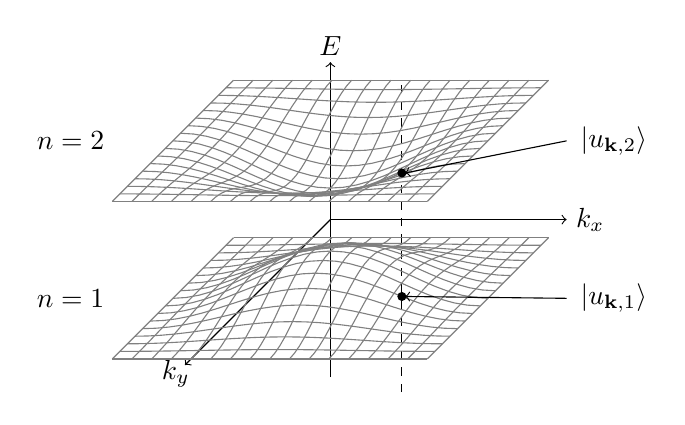
\begin{tikzpicture}

\def \size{3}
\def \vsize {2}
\def \ksize{2}
\def \stepnum {8}

\draw [->] (0,0) -- (\size,0,0);
\draw  [->] (0,-\vsize,0) -- (0,\vsize,0);
\draw  [->] (0,0) -- (0,0,1.6*\size);

\draw node at (1.1*\size,0,0) {$k_x$};
\draw node at (0,1.1*\vsize,0) {$E$};
\draw node at (0,0,1.7*\size) {$k_y$};

\draw node at (-1.1*\size , 1, 0) {$n=2$};
\draw node at (-1.1*\size , -1, 0) {$n=1$};

\def \xone {0.5}
\def \yone {1.1}

\draw [dashed] (\yone, -2 ,\xone) -- (\yone, 2 ,\xone);



\foreach \yy in {-\stepnum, ..., \stepnum}
{	
	\def \y {\yy*(\ksize/\stepnum)}
	\draw [domain = -\ksize:\ksize, variable= \x, gray] plot ({\y},{0.15*(1+cos(\x*360/(2*\ksize)))*(1+cos(\y*360/(2*\ksize))) -1},{\x});
	\draw [domain = -\ksize:\ksize, variable= \x, gray] plot ({\x},{0.15*(1+cos(\x*360/(2*\ksize)))*(1+cos(\y*360/(2*\ksize))) -1},{\y});
	
	\draw [domain = -\ksize:\ksize, variable= \x, gray] plot ({\y},{-0.15*(1+cos(\x*360/(2*\ksize)))*(1+cos(\y*360/(2*\ksize))) +1},{\x});
	\draw [domain = -\ksize:\ksize, variable= \x, gray] plot ({\x},{-0.15*(1+cos(\x*360/(2*\ksize)))*(1+cos(\y*360/(2*\ksize))) +1},{\y});
}


\draw[fill] ({\yone},{0.15*(1+cos(\xone*360/(2*\ksize)))*(1+cos(\yone*360/(2*\ksize))) -1},{\xone}) circle [radius=0.05];
\draw[fill] ({\yone},{-0.15*(1+cos(\xone*360/(2*\ksize)))*(1+cos(\yone*360/(2*\ksize)))+1},{\xone}) circle [radius=0.05];

\draw [->] (3,-1,0) --  ({\yone+0.04},{0.15*(1+cos(\xone*360/(2*\ksize)))*(1+cos(\yone*360/(2*\ksize))) -1},{\xone}) ;
\draw [->] (3,1,0) -- ({\yone+0.04},{-0.15*(1+cos(\xone*360/(2*\ksize)))*(1+cos(\yone*360/(2*\ksize))) +1},{\xone}) ;

\draw node at (1.2*\size,-1,0) {$\ket{u_{\bf k, 1}}$};
\draw node at (1.2*\size,1,0) {$\ket{u_{\bf k, 2}}$};


\end{tikzpicture}
\end{center}

This diagram shows the example for a system with two distinct bands, shown as the grey mesh plots. At each point in the bands there exists a corresponding $\ket{u_{\bf k , n}}$ state. 



\subsection{Wannier States}\label{sec:wannier_states}
Using Bloch's theorem, we have shown that it is straightforward to construct a set of energy eigenstates, separated into bands. These eigenstates are tightly localised in Fourier space, and so must as a result be delocalised across the whole system in real space. For each band in our system we have a set of states covering the whole of $k$-space. Thus it seems natural to ask whether these states can be combined to produce a basis of states that are delocalised in Fourier space, but localised in real space. Such states are called Wannier states, a  comprehensive review of these states may be found in \cite{marzari_maximally_2012}. \par
For each band, a set of Wannier states may be constructed by taking the Fourier transform of the complete set of energy eigenstates in that band, according to
\begin{align}
	\ket{w_{\bf R, n}} = \frac{V_{\textup{u.c.}}}{(2 \pi)^d } \int _{\textup{BZ}} d\bf k\; e^{-i \bf k \cdot \bf R + i \alpha(\bf k)} \ket{\psi _{\bf k, n}},
\end{align}
where $ V_{\textup{u.c.}}$ is the volume of the unit cell, $\bf R$ denotes a vector in the Bravais lattice, and $\alpha $ denotes an arbitrary gauge transformation that may be applied to the states. In practice, we usually work in systems with periodic boundaries. This means that the $\bf k$-states are restricted to lie on a lattice and the expression becomes
\begin{align}
	\ket{w_{\bf R, n}} = \frac{1}{\sqrt N } \sum _{\bf k}  e^{-i \bf k \cdot \bf R + i \alpha(\bf k)} \ket{\psi _{\bf k, n}}.
\end{align}
This construction represents a unitary transformation of the basis of energy eigenstates, thus the Wannier states also form an orthonormal complete basis set for the band. This means that the projector onto that band may be equivalently expressed in terms of Wannier states,
\begin{align}
	\hat P = \sum_{\bf k} \ket{\psi _{\bf k, n}}\bra{\psi _{\bf k, n}} \equiv \sum_{\bf R} \ket{w_{\bf R, n}} \bra{w_{\bf R, n}}.
\end{align}
Furthermore it can be shown that the states are related by translation,
\begin{align}
	\braket{\bf m | w_{\bf R, n} } = \braket{\bf m + \bf L | w_{\bf R + \bf L, n} },
\end{align}
for any lattice vector $\bf L$.\par
Although a gauge transformation does not have a measurable effect on the Bloch states, it does in fact have a strong effect on the Wannier states. This is because the choice of gauge allows us to control how localised our Wannier states are. If we are able to find a smooth gauge -- where $\ket{\psi_{\bf k, n}}$ is an analytic function of $\bf k$ -- we end up with a set of exponentially localised Wannier functions \cite{cloizeaux_energy_1964}. However if it is not possible to find a smooth gauge over the Brillouin zone, then we have an obstruction to finding a tightly localised set of Wannier states.\par


\section{Abelian Berry Phase, Chern Number and Topology} \label{sec:chern_number}
%!TEX root = ./main.tex

In this section we will introduce the concepts of Berry phase, Berry flux and Chern number, quantities that will be of fundamental importance when trying to understand the properties of topological insulators. Berry phase was first introduced in \cite{berry_quantal_1984}, the ideas presented here will largely follow \cite{asboth_short_2016}, but other resources for understanding these concepts can be found in \cite{resta_geometry_2020,bohm_geometric_2003}. These concepts will first be introduced in the discrete case, looking at the Berry phase accumulated as one moves adiabatically around a lattice of quantum states. However in \textsection\ref{sec:continuous_case} we will extend the argument to include adiabatic paths around a smooth manifold of states. In \textsection\ref{sec:an_example} we will give a brief example of such a calculation, demonstrating how these concepts may be applied to periodic quantum systems.

\subsection{Discrete Case}

Suppose we have a quantum system that lives in a Hilbert space $\mathcal{H}$. States in this system are denoted by an equivalence class of vectors in this space. This means that two states that differ only by a complex phase still represent the same state,
\begin{align}
    \ket{\psi} \sim e^{-i\alpha}\ket{\psi}.
\end{align}
Thus we essentially have a degeneracy in our description of the physics taking place. It is possible to make a gauge transformation -- shifting the state by some complex phase -- without affecting the system in any measurable way.\par
Now suppose that we have collected a set of states that live in this Hilbert space, $\{ \ket{\psi_j}\}$. Rather than acting on each state with the same phase (and thus implementing a global gauge transformation), you apply a different phase to each state. This amounts to making a local gauge transformation,
\begin{align}
    \ket{\psi_j} \rightarrow e^{-i\alpha_j}\ket{\psi_j}.
\end{align}
The physical meaning of each state must be unaffected, so we expect that any quantity of physical importance should be invariant to our choice of gauge. With this condition in mind we can try to define quantities that compare our states, and test whether their definitions respect gauge invariance. The first quantity we propose is the relative phase between two states.
\begin{align}
    e^{-i\gamma_{j,k}} = \frac{\braket{\psi_j|\psi_k}}{|\braket{\psi_j|\psi_k}|}
\end{align}
Clearly this quantity is invariant under global gauge transformations, but it is definitely not invariant under a local transformation since it changes according to
\begin{align}
    e^{-i\gamma_{j,k}} \rightarrow e^{-i(\gamma_{j,k}+\alpha_j - \alpha_k)}.
\end{align}
Let's try something else.\par
We pick a set of $N$ ($\geq 3$) states $\ket{\psi_j}$ and arrange them in a loop.
\begin{center}
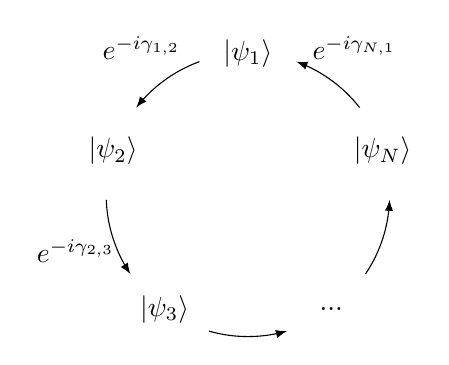
\begin{tikzpicture}

\def  \angoff {20}
\def \picsize {1.8}
\def \edistance {0.5}
\def \anground {72}

\draw [-latex,domain = \angoff:\anground-\angoff] plot ({\picsize * cos (\x + 90)}, {\picsize * sin (\x + 90)});
\draw [-latex,domain = \angoff:\anground-\angoff] plot ({\picsize * cos (\x + 90+\anground)}, {\picsize * sin (\x + 90+\anground)});
\draw [-latex,domain = \angoff:\anground-\angoff] plot ({\picsize * cos (\x + 90+2*\anground)}, {\picsize * sin (\x + 90+2*\anground)});
\draw [-latex,domain = \angoff:\anground-\angoff] plot ({\picsize * cos (\x + 90+3*\anground)}, {\picsize * sin (\x + 90+3*\anground)});
\draw [-latex,domain = \angoff:\anground-\angoff] plot ({\picsize * cos (\x + 90+4*\anground)}, {\picsize * sin (\x + 90+4*\anground)});

\draw node at (90:\picsize) {$\ket{\psi_1}$};
\draw node at (90+\anground:\picsize) {$\ket{\psi_2}$};
\draw node at (90+2*\anground:\picsize) {$\ket{\psi_3}$};
\draw node at (90+3*\anground:\picsize) {$...$};
\draw node at (90+4*\anground:\picsize) {$\ket{\psi_N}$};

\draw node at (90+0.5*\anground:\picsize+\edistance) {$e^{-i \gamma_{1,2}}$};
\draw node at (90+1.5*\anground:\picsize+\edistance) {$e^{-i \gamma_{2,3}}$};
\draw node at (90+4.5*\anground:\picsize+\edistance) {$e^{-i \gamma_{N,1}}$};

\end{tikzpicture}
\end{center}
We can now define a new quantity called the Berry phase:
\begin{align}\label{berry1}
    e^{-i \gamma^{B}} = \frac{\braket{\psi_1|\psi_2}\braket{\psi_2|\psi_3}...\braket{\psi_N|\psi_1}}{|\braket{\psi_1|\psi_2}\braket{\psi_2|\psi_3}...\braket{\psi_N|\psi_1}|}
\end{align}
Another way of writing this would be
\begin{align}
    \gamma^{B} = -\arg \tr \left[ \rho_{1} \;\rho_{2} \; ... \;\rho_{N} \right ],
\end{align}
where trace is over the whole system, and the $\rho$ states are density matrices
\begin{align}
    \rho_{i} = \ket{\psi_{i}}\bra{\psi_{i}}.
\end{align}
This quantity is clearly gauge-invariant, since any phase you attach to a state $\ket{\psi_m}$ will show up twice, once from $\braket{\psi_m|\psi_{m+1}}$ and once from $\braket{\psi_{m-1}|\psi_{m}}$. The phase will have opposite sign in each of these expressions so they cancel out. Furthermore, we can see that the Berry phase around a loop is simply the sum of all the relative phases around that loop modulo $2\pi$.
\begin{align}
	\gamma^B = \sum_{n=1}^N \gamma_{n,n+1} \mod 2\pi
\end{align}


\subsubsection{Berry Flux}

We now imagine that we have some massive amount of states arranged in a grid. These are labeled according a pair of parameters that we will call $q_x$ and $q_y$, $\ket{\psi_{q_x,q_y}}$. Note that we have used $q$ as a label here because it will turn out that in periodic quantum systems, these states correspond to the Bloch eigenstates, and $q$ will correspond to the $\bf k$ parameter in our $\ket {u_{\bf k, n}}$ states.

\begin{center}
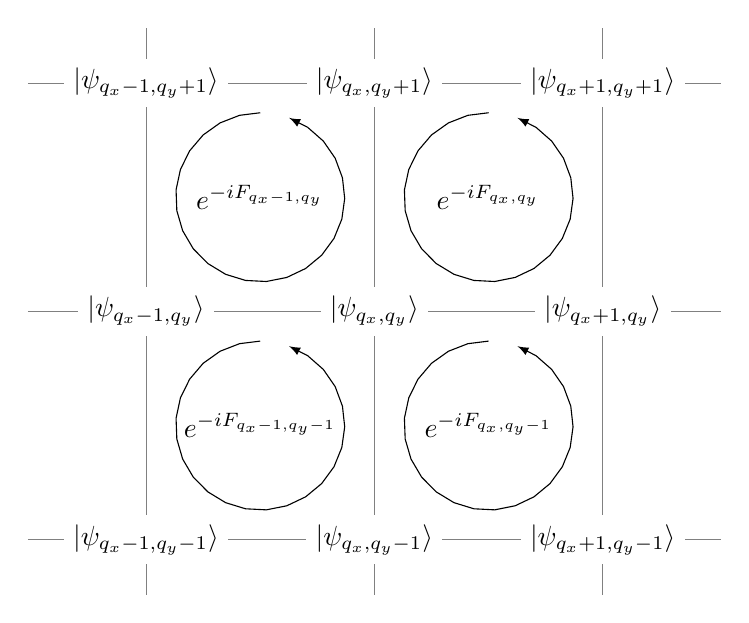
\begin{tikzpicture}

\def \gridsize{2.9}

\draw[step=\gridsize cm, help lines] (-\gridsize-1.5,-\gridsize-0.7) grid (\gridsize+1.5,\gridsize+0.7);
\draw node [fill= white] at (0,0) {$\ket{\psi_{q_x,q_y}}$};
\draw node [fill= white] at (\gridsize,0) {$\ket{\psi_{q_x+1,q_y}}$};
\draw node [fill= white] at (\gridsize,\gridsize) {$\ket{\psi_{q_x+1,q_y+1}}$};
\draw node [fill= white] at (0,\gridsize) {$\ket{\psi_{q_x,q_y+1}}$};
\draw node [fill= white] at (-\gridsize,0) {$\ket{\psi_{q_x-1,q_y}}$};
\draw node [fill= white] at (0,-\gridsize) {$\ket{\psi_{q_x,q_y-1}}$};
\draw node [fill= white] at (-\gridsize,-\gridsize) {$\ket{\psi_{q_x-1,q_y-1}}$};
\draw node [fill= white] at (\gridsize,-\gridsize) {$\ket{\psi_{q_x+1,q_y-1}}$};
\draw node [fill= white] at (-\gridsize,\gridsize) {$\ket{\psi_{q_x-1,q_y+1}}$};

\draw [-latex, domain = 0:340] plot ({0.37 *\gridsize* cos (\x + 90) + 0.5 * \gridsize }, {0.37 *\gridsize* sin (\x + 90) + 0.5 *\gridsize });
\draw [-latex, domain = 0:340] plot ({0.37 *\gridsize* cos (\x + 90) - 0.5 * \gridsize }, {0.37 *\gridsize* sin (\x + 90) + 0.5 *\gridsize });
\draw [-latex, domain = 0:340] plot ({0.37 *\gridsize* cos (\x + 90) + 0.5 * \gridsize }, {0.37 *\gridsize* sin (\x + 90) - 0.5 *\gridsize });
\draw [-latex, domain = 0:340] plot ({0.37 *\gridsize* cos (\x + 90) - 0.5 * \gridsize }, {0.37 *\gridsize* sin (\x + 90) - 0.5 *\gridsize });

\draw node at (0.5*\gridsize, 0.5*\gridsize) {$e^{-i F_{q_x,q_y}}$};
\draw node at (0.5*\gridsize, -0.5*\gridsize) {$e^{-i F_{q_x,q_y-1}}$};
\draw node at (-0.5*\gridsize, 0.5*\gridsize) {$e^{-i F_{q_x-1,q_y}}$};
\draw node at (-0.5*\gridsize, -0.5*\gridsize) {$e^{-i F_{q_x-1,q_y-1}}$};

\end{tikzpicture}
\end{center}

We introduce a new quantity called the Berry flux. This is defined to be the Berry phase around a unit loop in our grid,
\begin{align}\label{eqn:berry_flux}
    F_{q_x,q_y} =  - \arg \tr \left[ \rho_{q_x,q_y} \;\rho_{q_x+1,q_y} \;\rho_{q_x+1,q_y+1} \;\rho_{q_x,q_y+1} \right ],
\end{align}
where each $\rho$ represents the density matrix
\begin{align}
    \rho_{q_x,q_y} = \ket{\psi_{q_x,q_y}}\bra{\psi_{q_x,q_y}}.
\end{align}
This quantity has a neat property. $F_{q_x,q_y}$ is just the sum (mod $2\pi$) of the relative phases along each edge of the plaquette starting at point $(q_x,q_y)$. Thus, if we wanted to calculate the Berry phase around some arbitrary loop that contained multiple plaquettes, we could just sum the value of $ F_{q_x,q_y} $ for every plaquette contained in that region. Each relative phase flips sign depending on which way round it is evaluated. Any internal edge is shared between two plaquettes and so will appear twice in the sum of Berry fluxes, with opposite signs. This means all internal edges have their contribution to the total phase cancelled out and we are left with the sum of the relative phases only around the boundary of our region.
\begin{align}\label{berry_sum_discrete}
     \exp \left[ {-i \sum_{\textup{ inside region}}F}\right ] = \exp\left [ -i\sum_{\textup{boundary}} \gamma\right ]
\end{align}
This vaguely resembles Stokes' law, however there is one subtlety worth mentioning. All we have required is that the complex exponential of each sum is the same. This does \textbf{not} mean that the sum of the Berry flux inside a region is equal to the sum of relative phases around the boundary, since they are allowed to differ by an arbitrary multiple of $2\pi$


\subsubsection{Chern Number} \label{sec:discrete_chern}
Now let's assume that our grid of points $(q_x,q_y)$ has periodic boundaries, with $1\leq q_x \leq N_x$ and $1 \leq q_y \leq N_y$. That is, we have wrapped our space up to make a torus. The product of all the Berry flux phases is now always equal to 1,
\begin{align}\label{torus_sum}
    \prod_{q_x=1}^{N_x}\prod_{q_y=1}^{N_y}e^{-i F_{q_x,q_y}} = 1.
\end{align}
This is because every edge in our grid is now an internal edge, so they all cancel out! Again, as before, this does not mean that the sum of all Berry fluxes in our system vanishes. It means that the sum must always equal some multiple of $2\pi$. This sum gives us the Chern number, which we will call $\mathcal Q$,
\begin{align}\label{eqn:discrete_chern_number}
    \mathcal Q = \frac{1}{2\pi} \sum_{q_x,q_y}F_{q_x,q_y}.
\end{align}
$\mathcal Q$ is necessarily restricted to integer values, since a non-integer value would contradict equation \ref{torus_sum}.\par


\subsection{Continuous Case}\label{sec:continuous_case}

Now we repeat the entire derivation, but applied to continuous quantum systems, rather than a discrete lattice of states. In this new system, rather than a grid of discrete states $\ket{\psi_{q_x, q_y}}$ we are working with some smooth parameter space $\mathcal{P}$ of states.
\begin{align}
    \ket{\psi(\bf q)}, \; \bf q \in \mathcal{P}
\end{align}
In this context, a local gauge transformation amounts to applying some $\bf q$-dependent phase $\alpha(\bf q)$ to all of the states in our system.
\begin{align}
	\ket{\psi(\bf q)} \rightarrow e^{-i\alpha(\bf q)}\ket{\psi(\bf q)}.
\end{align}
Before we continue, let us define what we mean by a \textit{smooth gauge}. This is a choice of gauge for our states that ensures that the $\bf q$-derivative of a state, $\nabla_{\bf q}\ket{\psi(\bf q)}$ is always well-defined. In general it is not always possible to pick a gauge that is globally smooth over all of $\mathcal{P}$, however it \textit{is} always possible to pick a locally smooth gauge around the neighbourhood of some point in $\mathcal{P}$\footnote{Do we need a more in depth justification of this statement? Or is it ok just to state this and move on?}.

\par

We now want to look at the relative phase between a state at $\bf q$ and another state that is infinitesimally displaced from it, at $\bf q + d \bf q$. This can be expressed as
\begin{align}
    e^{-i\Delta\gamma} = \frac{\braket{\psi(\bf q)|\psi(\bf q+d\bf q)}}{|\braket{\psi(\bf q)|\psi(\bf q+d\bf q)}|}.
\end{align}
In the limit of small $d\bf q$ we can express $\ket{\psi(\bf q+d\bf q)}$ to first order in $d\bf q$ as
\begin{align}
    \ket{\psi(\bf q+d\bf q)} = \ket{\psi(\bf q)} + d\bf q \cdot \nabla_{\bf q} \ket{\psi(\bf q)}.
\end{align}
Which means that
\begin{align}
    \braket{\psi(\bf q)|\psi(\bf q+d\bf q)} = 1 + \braket{\psi(\bf q) |d\bf q \cdot \nabla _{\bf q}|\psi(\bf q)}.
\end{align}
Now, noticing that $ \braket{\psi(\bf q) | \nabla_{\bf q} |\psi(\bf q)}$ is pure imaginary, it can be shown that
\begin{align}\label{A_def}
    \Delta \gamma &= i \braket{\psi(\bf q) | \nabla_{\bf q} |\psi(\bf q)} \cdot d\bf q \\
    &= \textbf{A} \cdot d\bf q
\end{align}
The quantity multiplying $d\bf q$ is the Berry connection $\textbf{A}(\bf q)$. Like the relative phase before, it is not a gauge-invariant quantity. Under a gauge transformation it changes according to
\begin{align} \label{eqn:gauge}
    \ket{\psi(\bf q)} \rightarrow e^{-i\alpha(\bf q)}\ket{\psi(\bf q)},\;\;\; \textbf{A}(\bf q) \rightarrow \textbf{A}(\bf q) - \nabla _{\bf q} \alpha(\bf q)
\end{align}
Essentially $\textbf{A}(\bf q)$ is telling you how the phase changes as you move away from each point in $\mathcal{P}$. \par
As you move around some closed path $\mathcal C$ in $\mathcal{P}$, the Berry connection allows you to figure out the total phase accumulated over this route, according to
\begin{align} \label{eqn:flux_loop}
    \gamma(\mathcal C) = \oint_{\mathcal C} \textbf{A} \cdot d\bf q.
\end{align}
The total phase around the loop \textit{is} gauge invariant, one can see this intuitively by realising that it is identical to the Berry phase from the discrete case, but in the limit where the discrete steps become arbitrarily close together. However it is also immediately clear from looking at eqn. \ref{eqn:flux_loop} that any contribution to $\bf A$ from a gauge transformation has the form of a total derivative as in eqn. \ref{eqn:gauge}, so will vanish when integrated over a closed loop.


\subsubsection{Berry Curvature}
We now want to define a quantity that looks like the Berry flux we defined earlier. We start by rewriting eqn. \ref{eqn:flux_loop} in the language of differential forms, defining the one-form
\begin{align}
	A = A_a d q^a.
\end{align}
The Berry phase around some infinitesimally small closed path $ \mathcal C$ can be expressed as
\begin{align} 
    \gamma(\mathcal C) = \oint_{\mathcal C} A.
\end{align}
Now we can use Stokes' theorem to re-express this as a surface integral over some region $\mathcal{R}$ that has the curve $\mathcal C$ as its boundary
\begin{align}
	\gamma(\mathcal C) = \int_{\mathcal{R}} dA,
\end{align}
where $dA$ is the exterior derivative of A, a quantity that we will call the Berry curvature, $B$,
\begin{align}
	B &= dA\\
	 &= \frac{\partial A_a}{\partial q^b} \; dq^b \wedge dq^a.
\end{align}
This calculation has one important caveat. It is only possible to apply Stokes' theorem when $A$ is smooth over the region $\mathcal{R}$. This means that we need to have already picked a smooth gauge for our states at least in the region we are integrating over! As stated before, this is always possible, but only because we have allowed the region $\mathcal R$ to be some small subregion of $\mathcal P$.\par
The Berry curvature is a gauge-independent quantity, as can be seen by substituting the gauge-transformed form of $A$ (eqn. \ref{eqn:gauge}) into the definition. \par
Now, in a two dimensional parameter space, this integral becomes
\begin{align}
	\gamma(\mathcal C) = \int_{\mathcal{R}} d q_x\, d q_y \left (  \partial_{x} A_{y}(\bf q) - \partial_{y} A_{x}(\bf q) \right ),
\end{align}
and we can see that the Berry curvature is a scalar
\begin{align}
	B = \partial_{x} A_{y}(\bf q) - \partial_{y} A_{x}(\bf q).
\end{align}
Similarly in three dimensions the Berry curvature is a vector quantity
\begin{align} \label{eqn:3d_curvature}
    \textbf{B}(\textbf{q}) = \nabla_\textbf{q} \times \textbf{A}(\textbf{q}).
\end{align}

\subsubsection{Chern Number}

As in \textsection\ref{sec:discrete_chern}, we make the assertion that the parameter space $\mathcal P$ is a closed manifold such as a torus. The Chern number is defined as the integral of the Berry curvature across the whole parameter space
\begin{align}
    \mathcal Q &= \frac{1}{2\pi} \int_{\mathcal{P}} B.
\end{align}
In a two-dimensional parameter space $(q_x,q_y)$, this can be expressed as
\begin{align}
     &= \frac{1}{2\pi} \int_{\mathcal{P}}\left [ \partial_x \braket{\psi(\bf q) | \partial_y \psi(\bf q)} - \partial_y \braket{\psi(\bf q) | \partial_x \psi(\bf q)}\right ] \, dq_x\, dq_y\\
     &= \frac{1}{\pi} \Im  \int_{\mathcal{P}} \braket{\partial_x \psi(\bf q) | \partial_y \psi(\bf q)}\, dq_x\, dq_y
\end{align}
The Chern number here is also restricted to only take integer values. This can be seen by realising that the continuous system is equivalent to a lattice system in the limit where the lattice spacing tends to zero, and so the same argument applies. A more careful justification can be found in \cite{vanderbilt_berry_2018}.

\subsection{An Example - The Two-Level System} \label{sec:an_example}

We will illustrate these concepts with the example of a two-state system. Our first step will be to parametrise the possible Hamiltonians in such a system using a vector $\bf d$. We will then solve this Hamiltonian for the positive and negative energy eigenstates. This allows us to look at how the eigenstates change as we smoothly deform the Hamiltonian, exploring the parameter space of $\bf d$. By examining how the eigenstates of $\hat H$ depend on the parametrisation, we can calculate the Berry curvature of the positive and negative energy states. We then connect this with our understanding of the Bloch states in a periodic quantum system. We discuss how the bulk Hamiltonian of a periodic system corresponds to the embedding of a closed surface in $\bf d$-space and describe how to calculate the Chern number of the bands in such a system.\par
Here the Hilbert space is $\mathbb{C}^2$. This means that any Hamiltonian we construct must be a $2\times 2$ Hermitian matrix. We will parametrise this in terms of a Pauli vector, $\bf d$,
\begin{align}
    H = \textbf{d}\cdot\hat{\sigma}  = d_i \sigma^i.
\end{align}
where the $\sigma_i$ are the Pauli matrices.\par
The set of possible Hamiltonians is thus a manifold in itself, $ \{H\} \cong \mathbb{R}^3 $, since $\textbf{d} \in \mathbb{R}^3 $. The first thing we will do is to express the vector $\textbf{d}$ in standard spherical polar coordinates, giving us a Hamiltonian that looks like
\begin{align}
    H = |\textbf{d}|\begin{pmatrix}
\cos(\theta) &e^{-i\phi}\sin{\theta} \\ 
 e^{i\phi}\sin{\theta}& -\cos(\theta)
\end{pmatrix}
\end{align}
This matrix has $H^2 = |\textbf{d}|^2 \1 $, so its eigenvalues are $\pm |\textbf{d}|$. One can show that its eigenvectors are
\begin{align}\label{states}
    \ket{+_{\textbf{d}}} = \begin{pmatrix}
e^{-i\phi/2}\cos(\theta/2)\\ 
e^{i\phi/2} \sin(\theta/2)
\end{pmatrix},\; \ket{-_{\textbf{d}}} = \begin{pmatrix}
-e^{-i\phi/2}\sin(\theta/2)\\ 
e^{i\phi/2} \cos(\theta/2)
\end{pmatrix}.
\end{align}
We have thus arrived at a set of states, $\ket {\pm_{\bf d}}$ that depend on some parameter $\bf d$. This means that we can apply what we just figured out in the last section. From eqn. \ref{eqn:3d_curvature} we can see that the Berry connection and Berry curvature of the $\ket +$ state is given by
\begin{align}
    \textbf{A}^\pm (\bf d) &= i\braket{\pm_\textbf{d} | \nabla_\textbf{d}| \pm_\textbf{d}}\\
    \textbf{B}^{\pm}(\bf d ) &= \nabla_\textbf{d} \wedge \textbf{A}^\pm (\bf d).
\end{align}
Using this equation it is possible to directly calculate the Berry curvature. We will omit this for the sake of brevity, however the full calculation can be found in Appendix \ref{sec:berry_curvature_two_level}. We arrive at the following expression for the Berry curvature of the $\ket +$ and $\ket -$ states:
\begin{align}
    \textbf{B}^{\pm} = \pm \frac{\hat{n}_\textbf{d}}{2\textbf{d}^2}
\end{align}
where $\hat{n}_\textbf{d}$ is a unit vector pointing in the direction of $\textbf{d}$.\par
The Berry curvature is equivalent to a monopole field radiating out from the origin in $\bf d$-space, in analogy with electrostatics. Now, suppose we wanted to calculate the Berry phase of the $\ket{+_{\bf d}}$ state around some path in $\bf d$-space, we would want to evaluate
\begin{align}
	\gamma^+ (C) = \oint_{\mathcal C} \bf A^+ (\bf d) \cdot d \bf d.
\end{align}
Re-expressing this in terms of the Berry curvature gives us
\begin{align}
	\gamma^+ (C) = \int_{\mathcal R} \bf B^+ (\bf d) \cdot d \bf S,
\end{align}
where the integral is over a region $\mathcal R$ that has the curve $\mathcal C$ as its boundary. Since the Berry curvature is just a monopole field with charge $\frac{1}{2}$, this integral ends up evaluating half the solid angle subtended by the curve $\mathcal C$.
\begin{equation}
    \gamma^+ (C) = \frac{1}{2}\Omega_{\mathcal{C}}.
\end{equation}

\subsubsection{Chern Number}

Now we can connect this with our understanding of Bloch states. We will work with a translationally symmetric lattice Hamiltonian in two-dimensional space. As we showed in section \ref{sec:lattice_bloch}, it is always possible to diagonalise this Hamiltonian in the plane-wave basis,
\begin{align}
	\hat H = \sum_{\bf k} \ket{\bf k}\bra{\bf k} \otimes \hat H (\bf k).
\end{align}
If the unit cell contains two sites, then $\hat H (\bf k)$ is a $2 \times 2$ matrix that depends on $\bf k$. We can write it in terms of a $\bf d$ vector that depends on $\bf k$.
\begin{align}
H(\textbf{k}) &= \textbf{d}(\textbf{k})\cdot \hat{\sigma}, \\
    \textbf{k} &= (k_x,k_y).
\end{align}
We know $\textbf{k}$ lives on the surface of a torus, since both $k_x$ and $k_y$ are periodic with some maximum value $k_{x}^{\textup{Max}}$ and $k_{y}^{\textup{Max}}$. Furthermore, $\textbf{d}$ (and by extension $\hat H$) live in the space $\mathbb{R}^3$. Thus, the mapping $\textbf{d}$ is
\begin{align}
    \textbf{d} : S^1 \times S^1 &\rightarrow \mathbb{R}^3 \\
    \textbf{d} : (k_x,k_y) &\mapsto \textbf{d}(\textbf{k})
\end{align}
The map is embedding a two-dimensional surface (the torus) into three-dimensional flat space ($\mathbb{R}^3$). There are no limits on how you can do this embedding, the torus can be as twisted and crinkled up as you like so long as the embedding respects the topology of the Brillouin zone (it can't include discontinuities or cuts or other abusive things).\par
When we want to calculate the Berry phase around a loop in k-space, all we have to do is look at the corresponding loop in d-space. Then we integrate the Berry connection over some surface that has this loop as its boundary. The Berry connection actually looks like a radiating monopole so we can simplify further, knowing that we just need to find the solid angle subtended by the curve around the origin and divide it by two.\par


\begin{center}
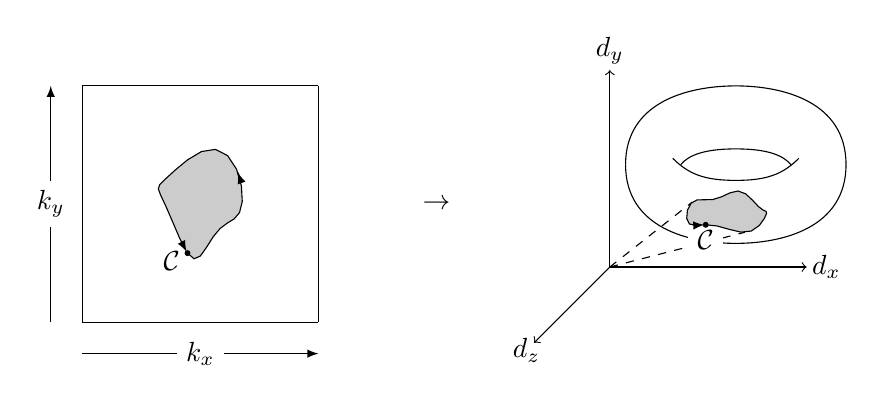
\begin{tikzpicture}

\def \axissize {2.5}
\def \squaresize{1.5}

\def \squarepos{-3}
\def \axisxpos {2.2}
\def \axisypos{-0.8}
\def \arrowdistance {0.4}

\draw (\squarepos - \squaresize , - \squaresize) -- (\squarepos + \squaresize, - \squaresize);
\draw (\squarepos + \squaresize , - \squaresize) -- (\squarepos + \squaresize, + \squaresize);
\draw (\squarepos + \squaresize , + \squaresize) -- (\squarepos - \squaresize, + \squaresize);
\draw (\squarepos - \squaresize , + \squaresize) -- (\squarepos - \squaresize, - \squaresize);

\draw [-latex] (\squarepos - \squaresize  , - \squaresize-\arrowdistance) -- (\squarepos + \squaresize, - \squaresize- \arrowdistance);
\draw [-latex] (\squarepos - \squaresize-\arrowdistance, - \squaresize) -- (\squarepos - \squaresize -\arrowdistance, + \squaresize) ;

\draw node [fill= white] at (\squarepos  , - \squaresize-\arrowdistance) {$k_x$};
\draw node [fill= white] at (\squarepos - \squaresize-\arrowdistance, 0)  {$k_y$};

\draw [-latex, fill= black!20, domain = 0:358] plot ({0.5 * (cos(\x-120) + 0.2 * sin(2*(\x-120))) + \squarepos},{0.6*(sin(\x-120) + 0.2 * cos(3*(\x-190))) });
\draw [-latex, domain = 160:161] plot ({0.5 * (cos(\x-120) + 0.2 * sin(2*(\x-120))) + \squarepos},{0.6*(sin(\x-120) + 0.2 * cos(3*(\x-190))) });

\draw[fill] ({0.5 * (cos(-120) + 0.2 * sin(2*(0-120))) + \squarepos},{0.6*(sin(-120) + 0.2 * cos(3*(-190))) }) circle [radius=0.03];
\draw node at ({0.5 * (cos(-120) + 0.2 * sin(2*(0-120))) + \squarepos -0.2 },{0.6*(sin(-120) + 0.2 * cos(3*(-190))) -0.1 }) {$\mathcal C$};


\draw node at (0,0) {$\huge \rightarrow$};

\draw [->] (\axisxpos,\axisypos,0) -- (\axisxpos+\axissize,\axisypos,0);
\draw  [->] (\axisxpos,\axisypos,0) -- (\axisxpos,\axisypos+\axissize,0);
\draw  [->] (\axisxpos,\axisypos,0) -- (\axisxpos,\axisypos,\axissize);

\def \donutscale {0.4}
\def \donutx {3.8}
\def \donuty {0.5}

\draw (-3.5*\donutscale+\donutx,0+\donuty) .. controls (-3.5*\donutscale+\donutx,2*\donutscale+\donuty) and (-1.5*\donutscale+\donutx,2.5*\donutscale+\donuty) .. (0+\donutx,2.5*\donutscale+\donuty);
\draw[xscale=-1] (-3.5*\donutscale-\donutx,0+\donuty) .. controls (-3.5*\donutscale-\donutx,2*\donutscale+\donuty) and (-1.5*\donutscale-\donutx,2.5*\donutscale+\donuty) .. (0-\donutx,2.5*\donutscale+\donuty);
\draw[rotate=180] (-3.5*\donutscale-\donutx,0-\donuty) .. controls (-3.5*\donutscale-\donutx,2*\donutscale-\donuty) and (-1.5*\donutscale-\donutx,2.5*\donutscale-\donuty) .. (0-\donutx,2.5*\donutscale-\donuty);
\draw[yscale=-1] (-3.5*\donutscale+\donutx,0-\donuty) .. controls (-3.5*\donutscale+\donutx,2*\donutscale-\donuty) and (-1.5*\donutscale+\donutx,2.5*\donutscale-\donuty) .. (0+\donutx,2.5*\donutscale-\donuty);
\draw (-2*\donutscale+\donutx,.2*\donutscale+\donuty) .. controls (-1.5*\donutscale+\donutx,-0.3*\donutscale+\donuty) and (-1*\donutscale+\donutx,-0.5*\donutscale+\donuty) .. (0+\donutx,-.5*\donutscale+\donuty) .. controls (1*\donutscale+\donutx,-0.5*\donutscale+\donuty) and (1.5*\donutscale+\donutx,-0.3*\donutscale+\donuty) .. (2*\donutscale+\donutx,0.2*\donutscale+\donuty);
\draw (-1.75*\donutscale+\donutx,0+\donuty) .. controls (-1.5*\donutscale+\donutx,0.3*\donutscale+\donuty) and (-1*\donutscale+\donutx,0.5*\donutscale+\donuty) .. (0+\donutx,.5*\donutscale+\donuty) .. controls (1*\donutscale+\donutx,0.5*\donutscale+\donuty) and (1.5*\donutscale+\donutx,0.3*\donutscale+\donuty) .. (1.75*\donutscale+\donutx,0+\donuty);

\def\spposx{3.7}
\def\spposy{-0.1}

\def \angone {280}
\def \angtwo {50}

\draw [dashed] (\axisxpos,\axisypos,0) -- ({0.5 * (cos(\angone-120) + 0.1 * sin(2*(\angone-20))) + \spposx},{0.23*(sin(\angone-120) + 0.2 * cos(4*(\angone-190))) +\spposy});
\draw [dashed]  (\axisxpos,\axisypos,0) -- ({0.5 * (cos(\angtwo-120) + 0.1 * sin(2*(\angtwo-20))) + \spposx},{0.23*(sin(\angtwo-120) + 0.2 * cos(4*(\angtwo-190))) +\spposy});

\draw  node [fill=white]  at ({0.5 * (cos(-120) + 0.1 * sin(2*(-20))) + \spposx},{0.23*(sin(-120) + 0.2 * cos(4*(-190))) +\spposy-0.2}) {$\mathcal C$};

\draw [-latex, fill= black!20, domain = 0:358] plot ({0.5 * (cos(\x-120) + 0.1 * sin(2*(\x-20))) + \spposx},{0.23*(sin(\x-120) + 0.2 * cos(4*(\x-190))) +\spposy});
\draw[fill] ({0.5 * (cos(-120) + 0.1 * sin(2*(-20))) + \spposx},{0.23*(sin(-120) + 0.2 * cos(4*(-190))) +\spposy}) circle [radius=0.03];


\draw node at (\axisxpos+1.1*\axissize,\axisypos,0){$ d_x$};
\draw  node at  (\axisxpos,\axisypos+ 1.1*\axissize,0){$ d_y$};
\draw  node at (\axisxpos,\axisypos, 1.1*\axissize){$d_z$};
\end{tikzpicture}
\end{center}
What about the Chern number? To calculate this all we need to do is integrate the Berry curvature across the whole surface of the torus in d-space. If the embedding of the torus does not contain the origin, then the value of this integral is necessarily zero. This is because the torus has an inside and an outside, everywhere that the surface is presented with the inside facing the origin we have a positive contribution to the integral, however when the outside is facing the origin we get a negative contribution. If the origin is outside the torus then we have exactly equal negative and positive contributions and everything cancels out!\par
Now suppose the torus is embedded such that it contains the origin, then we will have a surface that catches all of the Berry flux on its inside\footnote{Maybe you spotted this is not quite true, the torus is not a sphere so there will be some bits where there are outside faces presented to the origin, such as when you hit the hole in the doughnut! These will be cancelled out by the additional inside faces and so overall you still get $4\pi$.} and the solid angle subtended is $4\pi$! This means that the Chern number will be $+1$. Furthermore, you could imagine wrapping the torus around the origin twice, so that it effectively contains two origins, now the Chern number will be $+2$. You could turn it inside out and then wrap it around the origin too, that would give $\mathcal Q=-1$ and so on...

\subsection{Final Notes}

We close this chapter with an explanation of the consequences of Chern number in topological insulators.

\subsubsection{Smoothly Deforming the Hamiltonian}

Now suppose that we have a pair of quantum systems that live in the same Hilbert space, described by $\hat H_1$ and $\hat H_2$. Suppose both of these Hamiltonians represent insulating materials. This means that the bands in these materials are separated across all of the Brillouin zone by a band gap. We might want to ask the question: \textit{Is it possible to smoothly deform $\hat H _1$ into $\hat H_2$ without ever crossing a point where the bands touch and the material becomes conductive?} \par
The answer to this is that it is only possible if the bands of $\hat H_1$ and $\hat H_2$ have the same Chern numbers. This is because the Chern number is always restricted to have integer value, it cannot continuously change as we smoothly deform the Hamiltonian. In order to change the Chern number of a band we must somewhere cross a point where it is impossible to define a Chern number at all, allowing it to jump discontinuously when we leave that point. This is precisely what happens when two bands touch, the description of a single band becomes ill-defined and our calculation for Chern number stops working.\par
We can illustrate this with the example in \textsection\ref{sec:an_example}. Smoothly deforming our Hamiltonian amounts to changing the shape of the torus embedded in $\bf d$-space. If any point on the surface of the torus touches the origin, we have a pair of zero-energy states appearing in our system, this means the bands touch and the system is conductive. If the band has a Chern number of one, this means that the torus contains the origin. If we wanted to smoothly deform this to have zero Chern number, we would need to move the torus such that the origin was now outside. At some point in this deformation the torus surface will have to touch the origin, creating a conducting Hamiltonian at that point.\par
Thus we can classify all Hamiltonians according to the Chern number of their bands. It is always impossible to smoothly deform a Hamiltonian into one with a different Chern number while remaining insulating.\par
This allows us to make a rough justification for why conducting edge states must appear wherever we have a material with nonzero Chern number. Suppose we have a large material where the Hamiltonian is allowed to vary slowly over space, defined by $\hat H (\bf r)$. Now let's stay that in some region this Hamiltonian looks locally like it has non-zero Chern number, $\hat H _{\textup{topological}}$, but in a different, distant region it looks locally like it has zero Chern number, $\hat H _{\textup{trivial}}$. We expect that between these regions the Hamiltonian must be gradually transforming between $\hat H _{\textup{topological}}$ and $\hat H _{\textup{trivial}}$. As we have described, it is impossible for our Hamiltonian to make this transformation without creating a conducting surface somewhere between these two regions -- edge states must appear! Loosely speaking, we can view the vacuum as a zero Chern number material, which gives us an intuitive picture for why we might expect materials with non-zero Chern number to always have edge states appearing on their surface, where the Hamiltonian has to transition to the vacuum. 

\subsubsection{Chern Number and Globally Smooth Gauges}\label{sec:chern_smooth_gauge}
If you thought carefully about the gauge that we chose in equation \ref{states} you might notice that it has a problem, There is actually a discontinuity at $\phi = \pi$ where $e^{i\phi}$ suddenly jumps as you cross over to $\phi = -\pi$. This is no oversight, it turns out that it is actually completely impossible to define a globally smooth set of states $\ket{\psi(\textbf{d})}$ for any band that has nonzero Chern number!\par
This is because if $\ket{\psi(\textbf{d})}$ were continuous everywhere, then the Berry connection would also have to be continuous everywhere. This would mean that we could invoke Stokes' theorem when calculating the Chern number, 
\begin{align}
	\mathcal Q &= \frac{1}{2\pi}\int_{\mathcal P} B \\ 
	&= \frac{1}{2\pi}\int_{d \mathcal P} A. \label{eqn:always_zero}
\end{align}
The problem is that the Berry curvature integral is over the whole space $\mathcal P$. Since $\mathcal P$ is a closed manifold, it must have no boundary, so eqn. \ref{eqn:always_zero} must be equal to zero. Another way of understanding this is to realise that if you were to discretise this integral into a lattice of states, every edge would be an internal edge and the total would always have to be zero!\par
In this sense, the Chern number can be regarded as something like a measure of the amount of discontinuity that \textit{must} be present regardless of the gauge you choose for the space.



\section{The Qi-Wu-Zhang Model}\label{sec:QWZ}
%!TEX root = ./main.tex

For the rest of this document, we will use the Qi-Wu-Zhang (QWZ) model as our example for a topological insulator, first introduced in \cite{qi_topological_2006}. This is because the QWZ model is a simple toy model for a two-dimensional topological insulator with nearest-neighbour interactions on a square lattice.\par
 We work in a similar Hilbert space as that used in \textsection\ref{sec:lattice_bloch}, on a lattice of unit cells indexed by a two dimensional lattice vector $\bf m$, where each cell contains two sites -- the QWZ model has two bands. Thus the Hilbert space of the system is spanned by states of the form
\begin{align}
    \ket{\psi} = \ket{m_x} \otimes \ket{m_y} \otimes \ket{\alpha}.
\end{align}
The lattice has size $(L_x,L_y)$, so we have 
\begin{align}
    m_x \in \{ 0,...,L_x-1\}\\
    m_y \in \{ 0,...,L_y-1\}\\
    \alpha \in \{0,1\}.
\end{align}
The QWZ model is defined by three terms, a hopping between unit cells in the $x$-direction, a hopping in the $y$-direction, and a staggered on-site potential whose strength is determined by a parameter $u$.
\begin{align}
    \hat H &= \sum_{\bf m} \ket{\bf m+ 1_x}\bra{\bf m} \otimes \frac{\sigma_z + i\sigma_x}{2} + h.c. \nonumber \\
    &+ \sum_{\bf m} \ket{\bf m+ 1_y}\bra{\bf m} \otimes \frac{\sigma_z + i\sigma_y}{2} + h.c. \nonumber \\
    &+ \sum_{\bf m} \ket{\bf m}\bra{\bf m} \otimes u\; \sigma_z,
\end{align}
where $1_x$ and $1_y$ represent the unit displacement in their respective directions,
\begin{align}
	1_x = \begin{pmatrix}
	1\\
	0
	\end{pmatrix}, \ 1_y = \begin{pmatrix}
	0\\
	1
	\end{pmatrix}.
\end{align}
\begin{figure}[t]
\begin{center}
 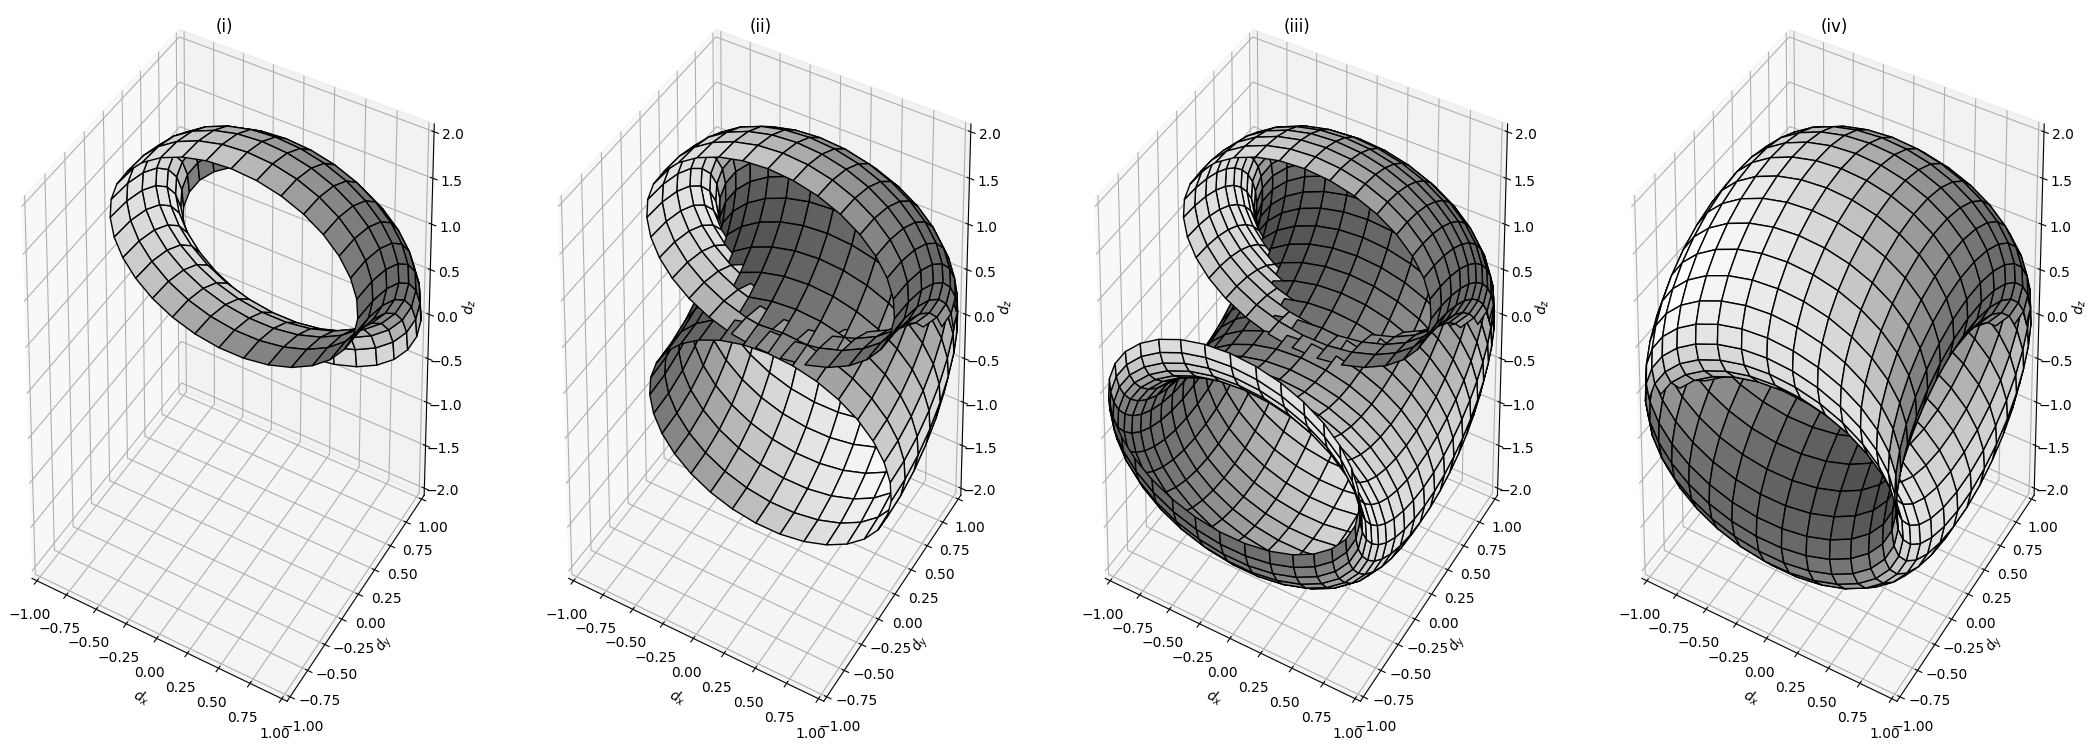
\includegraphics[width=\textwidth]{QWZ_donut}
\caption{The embedding of the Brillouin zone in $\bf d$-space for the QWZ model. This is shown in four progressive cutaways to ensure the internal structure can be seen. In all four images $k_x$ spans the interval $\left ( 0, 2\pi \right ]$, however in (i) $k_y$ spans $\left ( 0, \frac{\pi}{2} \right ]$, in (ii) $k_y$ spans $\left ( 0, \pi \right ]$, in (iii) $k_y$ spans $\left ( 0, \frac{3 \pi}{2} \right ]$, and in (iv) $k_y$ spans $\left ( 0, 2\pi \right ]$. }
\label{fig:QWZ_donut}
\end{center}
\end{figure}
Using Bloch's theorem, we can find the bulk Hamiltonian,
\begin{align}
    \hat H(\bf k) = \begin{pmatrix}
\sin k_x \\ 
\sin k_y\\ 
u + \cos k_x+ \cos k_y
\end{pmatrix} \cdot \bm \sigma.
\end{align}
Here, $k_x$ and $k_y$ determine our position in the Brillouin zone. As explained in \textsection\ref{sec:an_example}, this represents the embedding of a torus in $\bf d$-space, shown in fig. \ref{fig:QWZ_donut}.\par
The $u$-parameter has the effect of translating the torus by a fixed amount in the $z$-direction. From this we can see that the QWZ model only has non-zero Chern number for values of $u$ between -2 and 2. This is because translating the torus by any more than this will place the origin completely outside. The Chern number for the QWZ model is
\begin{align}
Q = \left\{\begin{matrix}
-1 &:&  -2 < u < 0 \\ 
1  &:&  0<u<2\\
0  &:&  \textit{otherwise} 
\end{matrix}\right. ,
\end{align}
not including the points at $u =$ -2, 0 and 2, at which the Chern number is undefined because the band gap closes and the material is conducting. Some example band structures for varying values of $u$ are shown in fig. \ref{fig:QWZ_band_struct}.
\begin{figure}[t]
\begin{center}
 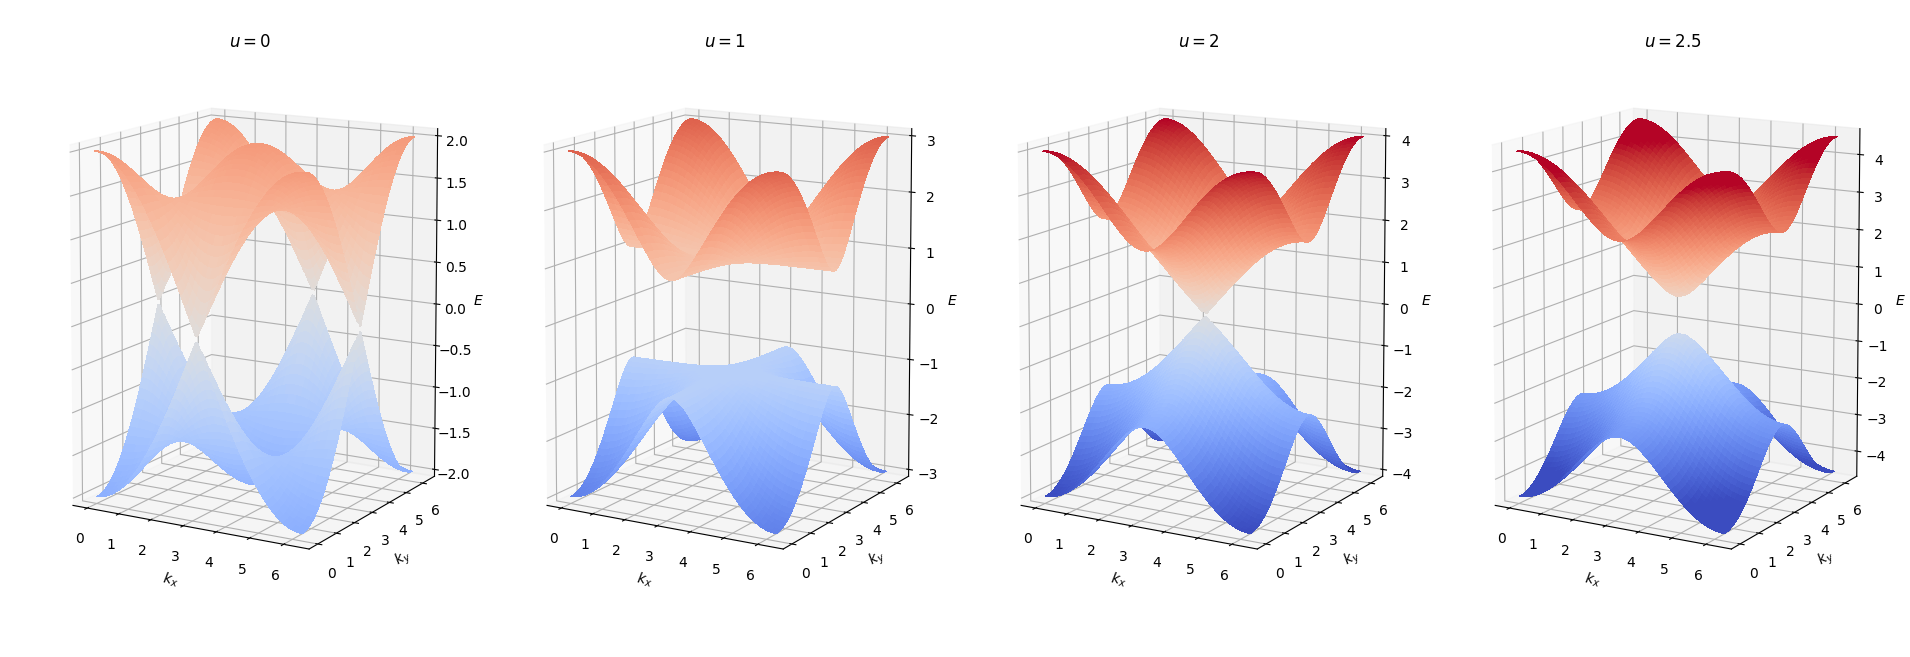
\includegraphics[width=\textwidth]{QWZ_band_struct}
\caption{Four examples of the band structure of the QWZ model are shown, for varying $u$ values between 0 and 2.5. At $u$ = 0 and 2, the bands touch and Chern number is undefined. At $u$ = 1, Q = +1, and at $u$ = 2.5, Q = 0.}
\label{fig:QWZ_band_struct}
\end{center}
\end{figure}

\subsection{Strip Geometry} \label{sec:QWZ_strip_geometry}
In much of the following discussion, we will be studying the QWZ model in a system with strip geometry. This means that the lattice is periodic and uniform in the $y$-direction, but is allowed to be non-uniform or have open boundaries in the $x$-direction. We will allow $u$ to vary in the $x$-direction, so add a subscript to indicate position-dependence $u \rightarrow u_{m_x}$. We can apply Bloch's theorem in the $y$-direction only, and our eigenstates take the following form,
\begin{align}
    \ket{\psi} = \ket{k_y}\otimes \ket{v_{k_y}^{n,l}},
\end{align}
where $\ket{k_y}$ is a plane wave solution
\begin{align}
    \ket{k_y} =\frac{1}{\sqrt{L_y}} \sum_{m_y} e^{i m_y k_y}\ket{m_y},
\end{align}
and $\ket{v_{k_y}^{n,l}}$ is a $2L_x$-element vector in the remaining part of the Hilbert space $\mathcal H_x \otimes \mathcal H_{\textup{int}} $. The $n$ index labels which band the state is in, and the $l$ index differentiates between the states in each band.
\begin{align}
    n &\in \{0,1\}\\
    l &\in \{ 0, \dots ,L_x -1\}.
\end{align}
The $v$-states are solutions of the semi-bulk Hamiltonian
\begin{align}
    \hat H(k_y) &= \sum_{m_x} \ket{m_x+1}\bra{m_x} \otimes \frac{\sigma_z + i\sigma_x}{2} + h.c.\nonumber \\
    &+ \sum_{m_x} \ket{m_x}\bra{m_x} \otimes \left [ (u_{m_x} + \cos k_y) \; \sigma_z + \sin k_y \; \sigma_y  \right ].
\end{align}
We have effectively reduced our system from a lattice of interacting sites in $x$ and $y$, to a set of chain models in $x$, that are each labelled by a value of $k_y$.
\begin{center}
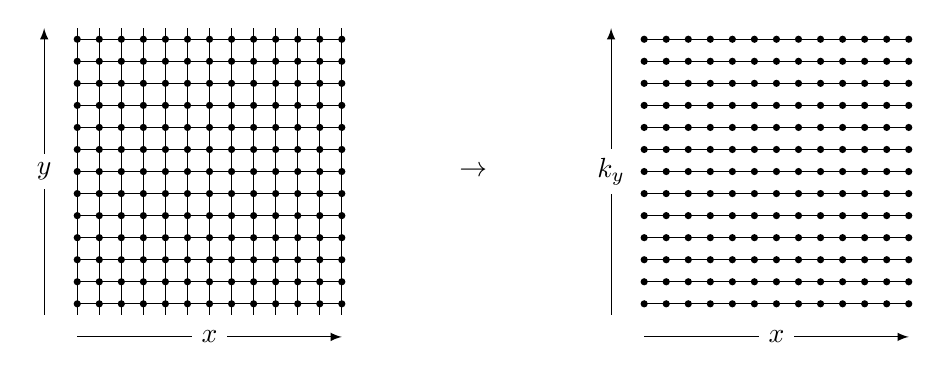
\begin{tikzpicture}

\def \cellsize{0.28}
\def \numcells{6}
\def \pos {3.6}

\foreach \x in {-\numcells, ..., \numcells}{
\draw [] (\x*\cellsize - \pos, -\numcells*\cellsize -0.5*\cellsize) -- (\x*\cellsize - \pos, \numcells*\cellsize + 0.5*\cellsize);
}
\foreach \y in {-\numcells, ..., \numcells}{
\draw [] (-\numcells*\cellsize -\pos, \y*\cellsize) -- (\numcells*\cellsize - \pos, \y*\cellsize);
} 

\foreach \x in {-\numcells, ..., \numcells}{
\foreach \y in {-\numcells, ..., \numcells}{
\fill[] (\x*\cellsize - \pos, \y*\cellsize) circle (1.3pt);
}
}

\draw [-latex] (-\numcells*\cellsize -\pos, -\numcells*\cellsize - 1.5*\cellsize) -- (\numcells*\cellsize - \pos, -\numcells*\cellsize - 1.5*\cellsize);
\draw node [fill= white] at (-\pos, -\numcells*\cellsize - 1.5*\cellsize) {$x$};

\draw [-latex] (-\numcells*\cellsize - 1.5*\cellsize - \pos, -\numcells*\cellsize -0.5*\cellsize) -- (-\numcells*\cellsize - 1.5*\cellsize - \pos, \numcells*\cellsize + 0.5*\cellsize);
\draw node [fill= white] at  (-\numcells*\cellsize - 1.5*\cellsize - \pos, 0) {$y$};

\draw node at (-0.25,0) {$\huge \rightarrow$};


\foreach \y in {-\numcells, ..., \numcells}{
\draw [] (-\numcells*\cellsize +\pos, \y*\cellsize) -- (\numcells*\cellsize + \pos, \y*\cellsize);
} 

\foreach \x in {-\numcells, ..., \numcells}{
\foreach \y in {-\numcells, ..., \numcells}{
\fill[] (\x*\cellsize + \pos, \y*\cellsize) circle (1.3pt);
}
}

\draw [-latex] (-\numcells*\cellsize +\pos, -\numcells*\cellsize - 1.5*\cellsize) -- (\numcells*\cellsize + \pos, -\numcells*\cellsize - 1.5*\cellsize);
\draw node [fill= white] at (+\pos, -\numcells*\cellsize - 1.5*\cellsize) {$x$};

\draw [-latex] (-\numcells*\cellsize - 1.5*\cellsize + \pos, -\numcells*\cellsize -0.5*\cellsize) -- (-\numcells*\cellsize - 1.5*\cellsize+ \pos, \numcells*\cellsize + 0.5*\cellsize);
\draw node [fill= white] at  (-\numcells*\cellsize - 1.5*\cellsize + \pos, 0) {$k_y$};

\end{tikzpicture}
\end{center}
We can rewrite this, in terms of the $2\times2$ matrices $A$ and $B$,
\begin{align}
    A &= (u + \cos k_y) \; \sigma_z + \sin k_y \; \sigma_y,  \\ 
    B &= \frac{\sigma_z + i\sigma_x}{2},
\end{align}
and express our wavevectors in terms of a set of $L_x$ two-element states $\psi_n$
\begin{align}
    \ket{\psi} = \begin{pmatrix}
    \psi_0 \\
    \psi_1 \\
    \vdots \\
    \psi_{L_x -1}
     \end{pmatrix},
\end{align}
to arrive at a set of equations for the eigenvalues of the semi-bulk Hamiltonian.
\begin{align}
    \textup{Bulk:} &\ A\psi_n + B\psi_{n+1} + B^\dag \psi_{n-1} = \lambda \psi_n \\
    \textup{Left Edge:} &\ A\psi_1 + B\psi_{2} = \lambda \psi_1\\
    \textup{Right Edge:} &\ A\psi_{L_x} + B^\dag \psi_{L_x-1}  = \lambda \psi_n
\end{align}
The band structure for this system in both periodic boundaries and strip geometry is shown in fig. \ref{fig:strip_energy}.
\begin{figure}[t]
\begin{center}
 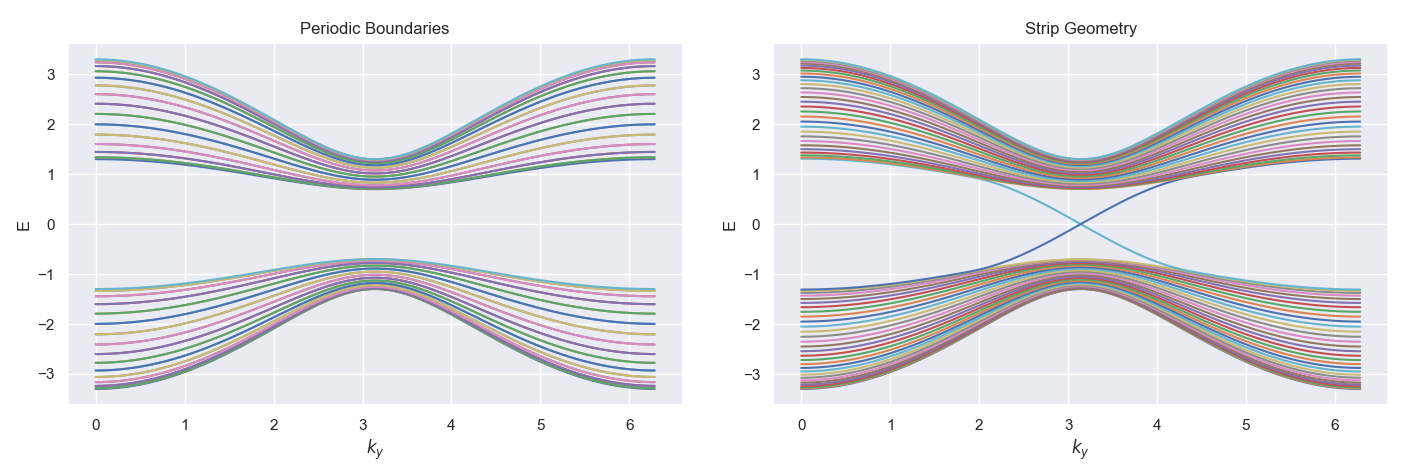
\includegraphics[width=.85\textwidth]{strip_energy}
\caption{An example band structure for a QWZ model with $u$ = 1.3 and $L_x$ = 30. On the left is the example for periodic boundary conditions, showing two well-separated bands. On the right is the case for open boundary conditions. Two edge states are shown leaving the bulk and crossing the gap, with the descending state being a left edge state, and the ascending state being a right edge state. }
\label{fig:strip_energy}
\end{center}
\end{figure}
We can now look at solving this analytically for the bulk and edge states. We will omit this calculation and print only the form of the results, however a full derivation can be found in appendix \ref{sec:QWZ_model_appendix}. Note that edge states are only present for certain values of $k_y$, which can be seen in figure \ref{fig:strip_energy}, where the edge states only separate from the bulk in a region around $k_y = \pi$. \par
Edge states have the form
\begin{align}
    \ket{\psi^{\textup{left}}_{k_y}} = \sqrt{1-\xi_l^2}\sum_{m=1}^{L_x} \xi_l^{m-1}\ket m \otimes \begin{pmatrix}
    1\\
    -i
    \end{pmatrix}
\end{align}
where 
\begin{align}
    \xi_l &= -u - \cos k_y.
\end{align}
This state has energy
\begin{align}
    E_l &= -\sin k_y.
\end{align}
Similarly, the right edge state is given by
\begin{align}
    \ket {\psi^{\textup{right}}_{k_y}} = \sqrt{1-\xi_r^2} \sum_{m=1}^{L_x} \xi_r^{L_x-m} \ket m \otimes  \begin{pmatrix}
    1\\
    i
    \end{pmatrix}
\end{align}
with the extra conditions
\begin{align}
   	 \xi_r &= -u-\cos k \label{eqn:edge_condition}\\
	E_r &= \sin k.
\end{align}
These edge states are only valid solutions for $k_y$ in the region
\begin{align}
	-1 < u+\cos k_y < 1.
\end{align}
These limits can be seen in fig. \ref{fig:strip_energy}, where the edge states peel away from the bands to cross the energy gap.\par
The bulk states are less straightforward to obtain exact solutions for, we give the general form for them and leave the details to appendix \ref{sec:QWZ_model_appendix}.
\begin{align}
    \ket{\psi^\pm_{k_y} }= \frac{1}{\sqrt{L_x}}\sum \ket{m}  \otimes \left [ \alpha e^{i \theta m} \ket{\phi_{\theta}^{\pm}} + \beta e^{-i \theta m} \ket{\phi_{\theta}^{\pm *}} \right ],
\end{align}
where the exact values of $\theta$, $\alpha$, $\beta$ and $\ket{\phi_{\theta}^{\pm}} $ can be found by solving some fairly unpleasant equations.\par
Here we mention a final caveat, These calculations are only strictly valid in the limit of a large system. This is because we have made the assumption the edge states can be calculated by taking into consideration only one edge and ignoring the effect of the other. The edge states decay exponentially through the system, so we are relying on the assumption that the edge state has effectively decayed to nothing before reaching the other side. When this condition is relaxed the edge states are able to couple to one another. This has a two effects, the first being that at the crossing of edge states, our energy eigenvalues become positive and negative superposition states of both edge states. The other is that the left state coupling to the right state shifts their energy levels such that no states cross $E = 0$ -- there is no longer a crossing of energy levels for the left and right edge states.









\section{Local Chern Markers} \label{sec:local_chern_markers}
%!TEX root = ./main.tex

The methods outlined in \textsection \ref{sec:chern_number} have proved extremely effective for characterising a wide variety of materials \cite{haldane_model_1988}, as well as providing the foundations for the modern theory of polarisation \cite{resta_macroscopic_1999}. However the definition of Chern number used also suffers from some important limitations. This is because we are forced to work in Fourier space in order to construct the Berry curvature. It is only possible to work in Fourier space when the system in question has both perfectly uniform translational symmetry, as well as living in either periodic or infinite boundary conditions. This is a serious problem since every material we encounter in the real world will fail to satisfy at least one of these conditions! Furthermore, it is not possible to apply any of these methods to quantum systems with interactions, or to systems out of equilibrium.\par
One potential solution to these problems has been the development of local Chern indicators such as the Bott Index \cite{toniolo_equivalence_2017,loring_guide_2019} and the Chern marker \cite{bianco_mapping_2011}. The idea here is to re-express the definition of Chern number in terms of a set of operators that are local, and so do not rely on the transition to Fourier space to make sense. Such a quantity should be equivalent to calculating the Chern number using $ k$-states in the case of a translationally symmetric, periodic system; however would still be possible in contexts where these conditions have been relaxed, and the notion of $k$-space breaks down. This would afford the researcher tools with which to comment on the topological characteristics of materials that had previously been out of reach using the standard methods, such as amorphous crystals \cite{agarwala_topological_2017}, quasi-periodic lattices \cite{huang_theory_2018} and systems out of equilibrium \cite{caio_topological_2019,toniolo_time-dependent_2018}. \par
In this section we start by introducing two such quantities, the Bott index and the Chern marker, giving their definitions as well as explaining how they are related. In both cases, these quantities are somewhat unstable when taken out of contexts in which the Chern number has a straightforward definition, and display a number of unexpected characteristics not explained by our definition of Chern number. 

\subsection{Bott Index}
We will work with a lattice model, where unit cells are indexed by a vector of the form $(m_x,m_y)$. The lattice has size $(L_x,L_y)$, and we have set periodic boundary conditions. Sites are indexed by 
\begin{align}
	\ket{\bf m \alpha} = \ket{\bf m} \otimes \ket{\alpha},
\end{align} 
where $\bf m$ is a vector labelling the unit cell and $\alpha$ selects a site within the unit cell. We shall use a Hamiltonian that has translational symmetry, so we may apply Bloch's theorem to obtain the form of the energy eigenstates,
\begin{align}
	\hat H &= \sum_{\bf k} \ket{\bf k}\bra{\bf k}\otimes \hat H(\bf k) \\ 
	\ket{\psi_{\bf k, n}} &= \ket{\bf k} \otimes\ket {u_{\bf k, n}},
\end{align}
where $\ket {u_{\bf k, n}}$ are the eigenstates of $\hat H(\bf k)$ and the momentum states are defined as in \textsection\ref{sec:lattice_bloch},
\begin{align}
	\ket{\bf k} = \frac{1}{\sqrt{L_x L_y}} \sum_{\bf m} e^{i \bf m \cdot \bf k} \ket {\bf m},
\end{align}
and we assume that the system has a total of $\eta$ bands, so $n \in  \{1,...,\eta\}$. Henceforth we will assume that only the $n$\ts{th} band is occupied, so we can construct a projector onto the occupied subspace, $\hat P$, and its complement, $\hat Q$.
\begin{align}
	\hat P & = \sum_{\bf k} \ket{\psi_{\bf k, n}}\bra{\psi_{\bf k, n}} \\
	\hat Q & = \sum_{\bf k,\, m \neq n} \ket{\psi_{\bf k, m}}\bra{\psi_{\bf k, m}}.
\end{align}
We also introduce a pair of operators $e^{i \delta_x \hat x}$ and $e^{i \delta_y \hat y}$, 
with
\begin{align}
\delta_x = \frac{2\pi}{L_x} ,\  \delta_y = \frac{2\pi}{L_y}.
\end{align}
In order to understand the effect of these operators, we consider their effect on the plane wave states
\begin{align}
	e^{i \delta_x \hat x}\ket{\bf k} &= \frac{1}{\sqrt{L_x L_y}} \sum_{\bf m} e^{i \delta_x \hat x} e^{i \bf m \cdot \bf k} \ket {\bf m} \\
	& = \frac{1}{\sqrt{L_x L_y}} \sum_{\bf m} e^{i \bf m \cdot (\bf k + \boldsymbol{\delta}_x)} \ket {\bf m}\\
	& = \ket{\bf k + \boldsymbol \delta_x},
\end{align}
similarly
\begin{align}
	e^{i \delta_y \hat y}\ket{\bf k} = \ket{\bf k + \boldsymbol \delta_y } 
\end{align}
Here the symbols $\boldsymbol{\delta}_x$ and $\boldsymbol{\delta}_y$ represents a vector translation in $\bf k$-space,
\begin{align}
	\boldsymbol \delta_x = \begin{pmatrix}
	\delta_x \\
	0
	\end{pmatrix}, \ \boldsymbol \delta_y = \begin{pmatrix}
	0 \\
	\delta_y
	\end{pmatrix}.
\end{align}
Thus, these operators effect a translation in $\bf k$ space by the minimum step in the reciprocal lattice. \par
Now let's look at the effect of these operators on the projector $\hat P$,
\begin{align}
	e^{i \delta_x \hat x} \hat P e^{-i \delta_x \hat x}  &=  \sum_{\bf k} e^{i \delta_x \hat x}  \ket{\bf k} \bra{\bf k} e^{-i \delta_x \hat x}\otimes \ket{u_{\bf k, n}}\bra{u_{\bf k, n}} \\
	&=  \sum_{\bf k} \ket{\bf k +\boldsymbol{\delta}_x} \bra{\bf k +\boldsymbol{\delta}_x } \otimes \ket{u_{\bf k, n}}\bra{u_{\bf k, n}} \\
	&=  \sum_{\bf k} \ket{\bf k } \bra{\bf k } \otimes \ket{u_{\bf k-\boldsymbol{\delta}_x, n}}\bra{u_{\bf k-\boldsymbol{\delta}_x , n}},
\end{align}
where the last line follows from a redefinition of $\bf k$. This is allowed as we are summing over the whole Brillouin zone. For the sake of clarity later on, we will re-express the density operator $\ket{u_{\bf k, n}}\bra{u_{\bf k, n}}$ in the following form
\begin{align}
	\ket{u_{\bf k, n}}\bra{u_{\bf k, n}} = \hat u_{\bf k, n},
\end{align}\par
so we get
\begin{align} \label{eqn:p_identity}
	e^{i \delta_x \hat x} \hat P e^{-i \delta_x \hat x}  =  \sum_{\bf k} \ket{\bf k } \bra{\bf k } \otimes \hat u_{\bf k-\boldsymbol{\delta}_x, n}.
\end{align}
Now we have enough tools to introduce the definition of the Bott index!
\begin{align}\label{eqn:bott_index}
    B(\bf A) = -\frac{N}{2\pi} \sum_\alpha \Im \bra{\bf A \alpha} \log \left [ \hat U\hat V\hat U^\dag \hat V^\dag + \hat Q \right ]\ket{ \bf A \alpha}
\end{align}
Here $N$ denotes the total number of unit cells in the system and the log is a standard matrix logarithm, defined as
\begin{align}
	\log (M) = \sum_{k=1}^\infty (-1)^{k+1} \frac{(M-\1)^k}{k}.
\end{align}
The Bott index is a local indicator, $\bf A$ is a vector that selects which unit cell in the system we are looking at, and
\begin{align}
	\hat U  = \hat P e^{i \delta_x \hat x} \hat P \\
	\hat V  = \hat P e^{i \delta_y \hat y} \hat P.
\end{align}
To make sense of this expression, let us focus on the $ \hat U\hat V\hat U^\dag \hat V^\dag$ part only, writing this out explicitly gives us
\begin{align}
	 \hat U\hat V\hat U^\dag \hat V^\dag = \hat P e^{i \delta_x \hat x} \hat P e^{i \delta_y \hat y} \hat P e^{- i \delta_x \hat x} \hat P e^{-i \delta_y \hat y} \hat P.
\end{align}
We now add in the identity in the form $e^{i \delta_x \hat x} e^{-i \delta_x \hat x} $, as well as the corresponding expression for $y$, and regroup the equation, taking advantage of the fact that $\hat x$ and $\hat y$ commute, to get
\begin{align}
	 \hat U\hat V\hat U^\dag \hat V^\dag =  \hat P
	  \left [ e^{i \delta_x \hat x} \hat P e^{-i \delta_x \hat x} \right]
	  \left [ e^{i \delta_y \hat y} e^{i \delta_x \hat x} \hat P  e^{-i \delta_y \hat y} e^{- i \delta_x \hat x } \right]
	  \left [ e^{i \delta_y \hat y} \hat P e^{-i \delta_y \hat y } \right]
	 \hat P.
\end{align}
Using eqn.~\ref{eqn:p_identity} we can now rewrite this in terms of Bloch states to get
\begin{align}
	\hat U\hat V\hat U^\dag \hat V^\dag = \sum_{\bf k} \ket{\bf k } \bra{\bf k } \otimes  \hat u_{\bf k, n}  \hat u_{\bf k -\boldsymbol{\delta}_x , n}  \hat u_{\bf k-\boldsymbol{\delta}_x-\boldsymbol{\delta}_y, n}  \hat u_{\bf k-\boldsymbol{\delta}_y, n}  \hat u_{\bf k, n}.
\end{align}
Since the first and last $\hat u$ density operator in this expression are identical, we can rewrite this in terms of a trace to get
\begin{align}
	\hat U\hat V\hat U^\dag \hat V^\dag = \sum_{\bf k} \ket{\bf k } \bra{\bf k } \otimes  \ket {u_{\bf k, n}} \bra{u_{\bf k, n}} \cdot  \tr \left [ \hat u_{\bf k, n} \hat u_{\bf k -\boldsymbol{\delta}_x , n}  \hat u_{\bf k-\boldsymbol{\delta}_x-\boldsymbol{\delta}_y, n}  \hat u_{\bf k-\boldsymbol{\delta}_y, n} \right ].
\end{align}
If we compare this to the definition of Berry flux (eqn.~\ref{eqn:berry_flux}), we see that this reduces to
\begin{align}
	\hat U\hat V\hat U^\dag \hat V^\dag = \sum_{\bf k} \ket{\bf k } \bra{\bf k } \otimes  \ket {u_{\bf k, n}} \bra{u_{\bf k, n}} \cdot r_{\bf k} e^{-i F_{\bf k-\boldsymbol{\delta}_x-\boldsymbol{\delta}_y}},
\end{align}
where $r_{\bf k}$ is just some real number that we don't care about, arising from the $u$ states not being perfectly parallel to one another. This is promising, remember we are aiming to get a sum of $F_{\bf k}$ over the whole Brillouin zone. Thus in order to extract the term in the exponential we would like to take a log. However, we cannot simply log the expression in the form we have here. This is because it only has support on the occupied subspace,
\begin{align}
    \hat U\hat V\hat U^\dag \hat V^\dag \sim \begin{pmatrix}
M &0 \\ 
 0& 0
\end{pmatrix},
\end{align}
where $M$ just indicates the presence of a nonzero operator. The presence of a null space means a log of this matrix will diverge. To remedy this, we add in the $\hat Q$ projector, 
\begin{align}
    \hat U\hat V\hat U^\dag \hat V^\dag  + \hat Q \sim \begin{pmatrix}
M &0 \\ 
 0& \1
\end{pmatrix}.
\end{align}
Now we can safely take the log of this matrix, getting the following result
\begin{align}
	\log \left [ \hat U\hat V\hat U^\dag \hat V^\dag + \hat Q \right ] = \sum_{\bf k} \ket{\bf k } \bra{\bf k } \otimes  \ket {u_{\bf k, n}} \bra{u_{\bf k, n}} \cdot \left ( \log(r_{\bf k})-i F_{\bf k-\boldsymbol{\delta}_x-\boldsymbol{\delta}_y}\right ),
\end{align}
Next we trace out the internal degree of freedom and squeeze this expression between a pair of position states $\ket {\bf A}$, selecting some arbitrary unit cell in our system. 
\begin{align}
	\sum_\alpha \bra{\bf A \alpha}\log \left [ \hat U\hat V\hat U^\dag \hat V^\dag + \hat Q \right ]   \ket{\bf A \alpha} = \sum_{\bf k} |\braket{\bf A|\bf k}|^2 \cdot  \braket{u_{\bf k, n}|u_{\bf k, n} } \cdot \left ( \log(r_{\bf k})-i F_{\bf k-\boldsymbol{\delta}_x-\boldsymbol{\delta}_y}\right ).
\end{align}
We can show that $|\braket{\bf A|\bf k}|^2 = \frac{1}{N}$ and $\braket{u_{\bf k, n}|u_{\bf k, n} } = 1$. All that is left to do is take the imaginary part, 
\begin{align}
	\sum_\alpha \Im \bra{\bf A \alpha}\log \left [ \hat U\hat V\hat U^\dag \hat V^\dag + \hat Q \right ]   \ket{\bf A \alpha} = \frac{1}{N} \sum_{\bf k} - F_{\bf k-\boldsymbol{\delta}_x-\boldsymbol{\delta}_y} .
\end{align}
Now, redefining $\bf k$ and multiplying by $-\frac{N}{2\pi}$ gives us
\begin{align}
	-\frac{N}{2\pi} \sum_\alpha \Im \bra{\bf A \alpha}\log \left [ \hat U\hat V\hat U^\dag \hat V^\dag + \hat Q \right ]   \ket{\bf A \alpha} = \frac{1}{2\pi} \sum_{\bf k}  F_{\bf k}.
\end{align}
By comparing with eqn.~\ref{eqn:discrete_chern_number}, we can see that we have arrived at an expression for the Chern number!
\begin{align}
	\mathcal Q = -\frac{N}{2\pi} \sum_\alpha \Im \bra{\bf A \alpha}\log \left [ \hat U\hat V\hat U^\dag \hat V^\dag + \hat Q \right ]   \ket{\bf A \alpha} .
\end{align}
Thus we have shown that in the case of a translationally symmetric system with periodic boundaries, the Bott index evaluated at any point in our material always exactly calculates the Chern number. Before we show some example calculations, let us introduce one more quantity.

\subsubsection{A Different Interpretation}

There is also another way to intuitively understand where the Bott index comes from, this loosely reflects the arguments presented in \cite{hastings_almost_2010}. As we saw in \textsection\ref{sec:wannier_states}, it is possible to construct a set of spatially localised states (the Wannier states) from the energy eigenstates of each band. Furthermore, these states can only be exponentially localised when we are able to define a smooth gauge across the whole of the Brillouin zone. As explained in \textsection\ref{sec:chern_smooth_gauge}, a smooth gauge is only achievable when the system has trivial Chern number. This means that the presence of a nonzero Chern number necessarily results in an obstruction to constructing a set of tightly localised Wannier states.\par
 If we were able to fully decompose the states in $\hat P$ into a set of localised states, then the $\hat x$ and $\hat y$ operators would commute when acted on the subspace spanned by $\hat P$. This would mean that the operators $\hat P e^{i \delta_x \hat x}\hat P $ and $\hat P e^{i \delta_y \hat y}\hat P $ would commute, so the Bott index would vanish. Thus the Bott index can be seen as indicating whether there is an obstruction to constructing a fully localised set of Wannier states -- telling us wether the material has nonzero Chern number.

 
 
\subsection{Chern Marker}

The Chern marker was first introduced in \cite{bianco_mapping_2011}, however we will not restate the derivation that they used. Instead we will justify the Chern marker by showing that it can be obtained from the Bott index in the limit of large system size.\par
Our starting point is the expression for Bott index, eqn.~\ref{eqn:bott_index}. We start by multiplying $\hat U$  and $\hat V$ by complex phases $e^{-i \delta_x C_x}$ and $e^{-i \delta_y C_y}$. This has no effect on the value of the Bott index, since the phases have opposite sign in $\hat U ^\dag$ and $\hat V ^\dag$.
\begin{align}
	\hat U  \rightarrow \hat P e^{i \delta_x (\hat x - C_x)} \hat P \\
	\hat V  \rightarrow \hat P e^{i \delta_y (\hat y - C_y)} \hat P.
\end{align}
As the system size becomes large, the factors $\delta_x$ and $\delta_y$ will become infinitesimally small. Around the neighbourhood of the unit cell at position $(C_x, C_y)$, the term in the exponential will be small so we can Taylor expand it,
\begin{align}
	\hat U &=  \hat P + i \delta_x \hat P \hat x_C \hat P + O(\hat x_C^2)\\
	\hat V &= \hat P + i \delta_y \hat P \hat y_C \hat P + O(\hat y_C^2)
\end{align}
where we have relabelled $ \hat x - C_x= \hat x_C$ and $ \hat y - C_y= \hat y_C$.  Using these expressions, we can re-express the operator $\hat U\hat V\hat U^\dag \hat V^\dag$ up to second order in $\delta$ as\footnote{You might have noticed that we have omitted the $\delta_x^2$ and $\delta_y^2$ terms. This is justified because those terms involve only hermitian operators, such as $ \hat P \hat x_C \hat P \hat x_C \hat P$, and these give no contribution when we take the imaginary part later.}
\begin{align}
 	\hat U\hat V\hat U^\dag \hat V^\dag = \hat P  - \delta_x \delta_y \left (  \hat P \hat x_C \hat P \hat y_C \hat P  -  \hat P \hat y_C \hat P \hat x_C \hat P \right ) + O(\delta_x^2, \delta_y^2)
\end{align}
Now we use the identities 
\begin{align}
	\hat P + \hat Q &= \1\\
	\log \left [ \1 + \delta M \right ] & \simeq M, \textup{  for  } \delta \textup{ small} 
\end{align}
to show that
\begin{align}
	\log \left [ \hat U\hat V\hat U^\dag \hat V^\dag  + Q  \right ] \simeq - \delta_x \delta_y \left [  \hat P \hat x_C \hat P, \hat P \hat y_C \hat P  \right ]
\end{align}
We can now drop the constant shifts in $\hat x_C$ and $\hat y_C$, since these vanish due to the commutator. Inserting this into the expression for Bott index, we arrive at the form of the Chern marker,
\begin{align}
 	C(\bf A)  = -2\pi i \sum_\alpha \bra{\bf A \alpha} \left [  \hat P \hat x \hat P, \hat P \hat y \hat P  \right ]  \ket{\bf A \alpha} .
\end{align}
We have skipped taking the imaginary part by noticing that the commutator is anti-Hermitian, so all of its eigenvalues are imaginary anyway, allowing us to make the substitution $\Im \rightarrow -i $.\par
This calculation comes with one important caveat. The Chern marker has an extra property that the Bott index lacks. If the system in question has finite size, then the sum of the Chern number over the whole system vanishes. This is because the sum of $C(\bf A)$ over the system is given by
\begin{align}\label{eqn:chern_sum}
	\sum_{\bf A} C(\bf A) = - 2\pi i \, \tr  \left [  \hat P \hat x \hat P, \hat P \hat y \hat P  \right ] ,
\end{align}
and the trace of a commutator is always zero in a finite Hilbert space. 

\begin{figure}[p]
\begin{center}
 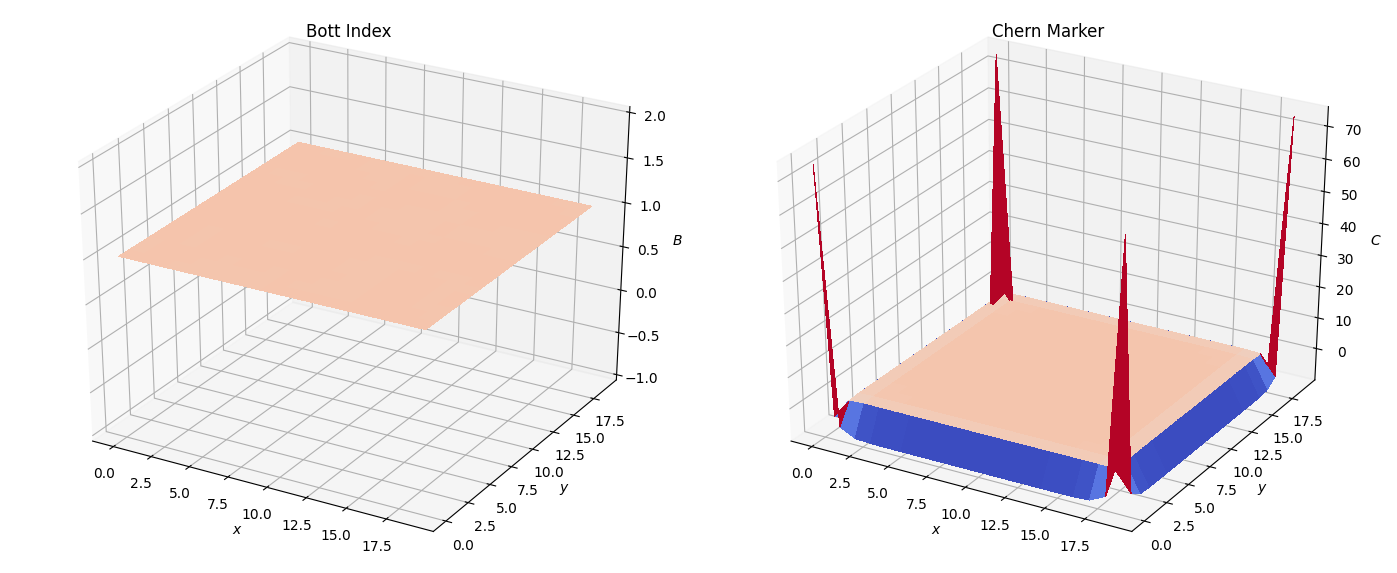
\includegraphics[width=\textwidth]{chern_bott_example}
\caption{The Bott index and Chern marker are calculated numerically for a QWZ material in periodic boundary conditions with constant $u = 1$ and $L_x = L_y = 20$.}
\label{fig:chern_bott_example}
\end{center}
\end{figure}
\begin{figure}[p]
\begin{center}
 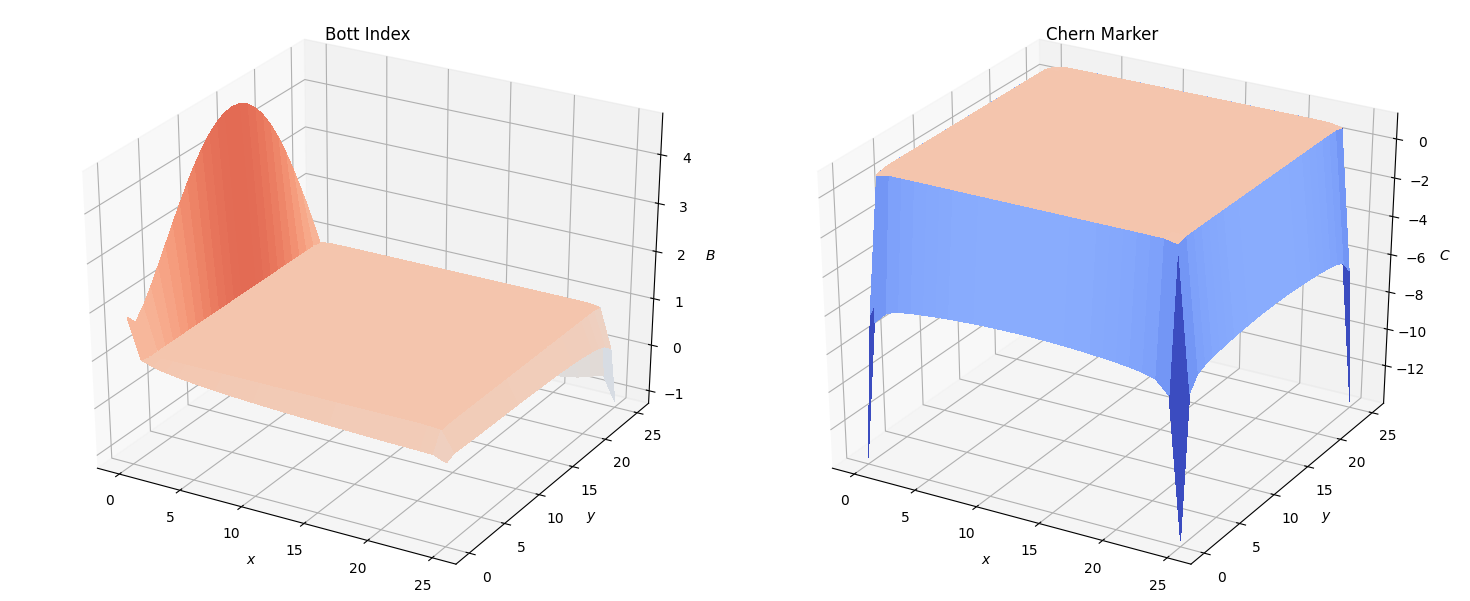
\includegraphics[width=\textwidth]{chern_bott_open}
\caption{The Bott index and Chern marker for a QWZ material with open boundaries with constant $u = 1$ and $L_x = L_y = 26$.}
\label{fig:chern_bott_open}
\end{center}
\end{figure}
\begin{figure}[p]
\begin{center}
 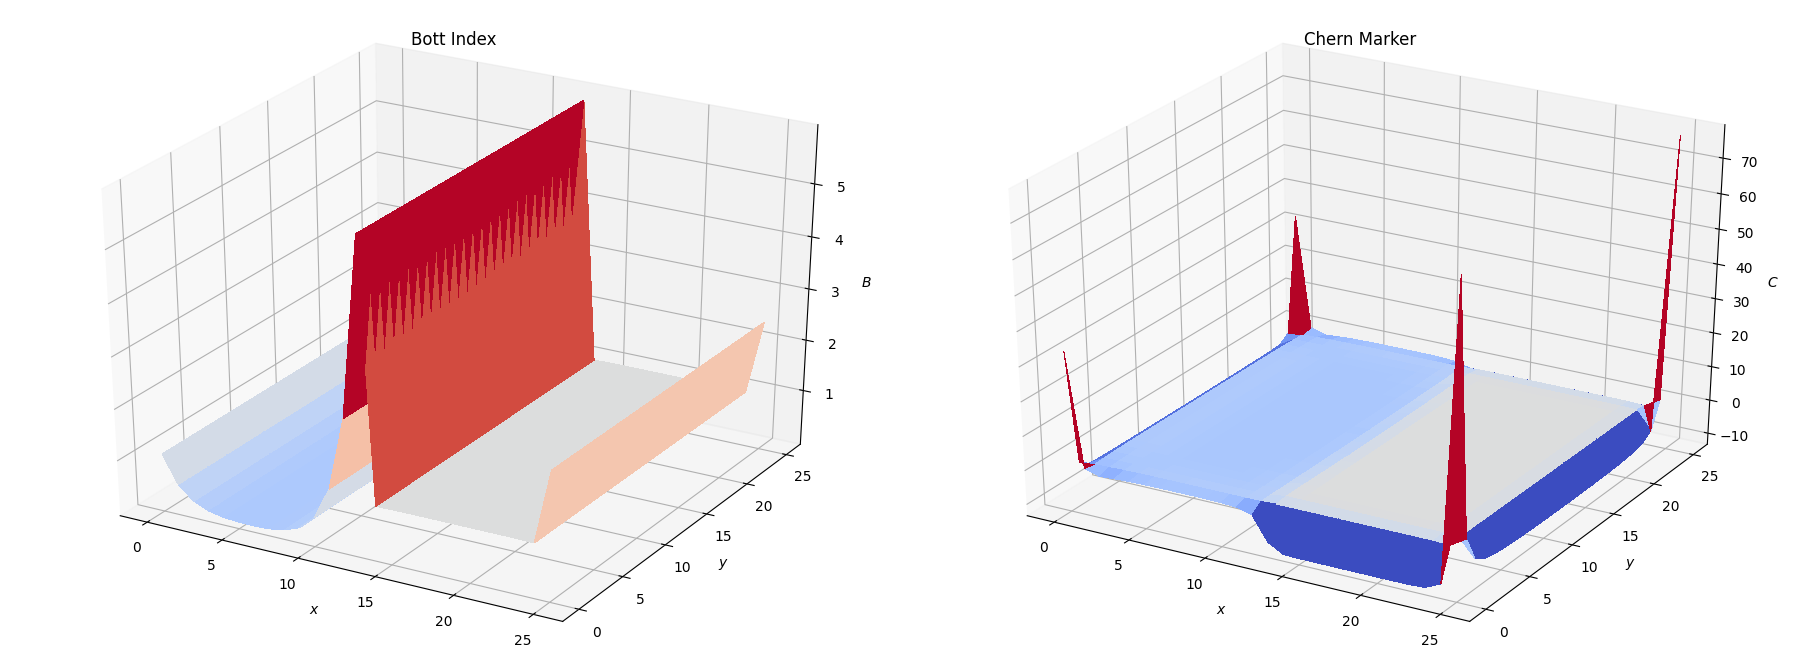
\includegraphics[width=\textwidth]{chern_bott_split_periodic}
\caption{The Bott index and Chern marker for a QWZ material with periodic boundaries with $u = 1$ for $x<13$ and $u = 2.5$ for  $x\geq13$, and $L_x = L_y = 26$. }
\label{fig:chern_bott_split_periodic}
\end{center}
\end{figure}
\begin{figure}[p]
\begin{center}
 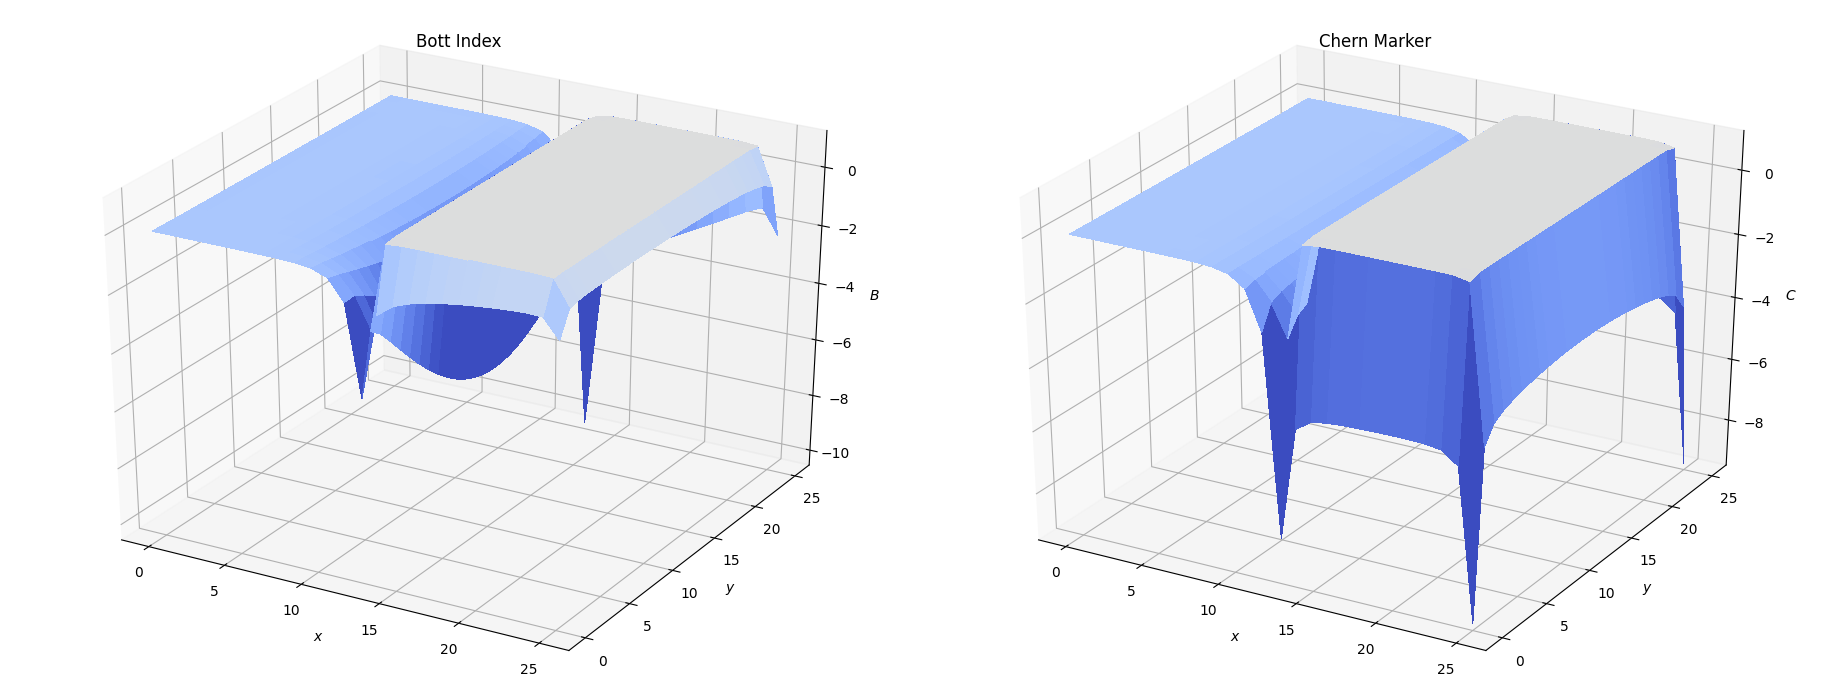
\includegraphics[width=\textwidth]{chern_bott_split_open}
\caption{The Bott index and Chern marker for a QWZ material with open boundaries with $u = 1$ for $x<13$ and $u = 2.5$ for  $x\geq13$, and $L_x = L_y = 26$. }
\label{fig:chern_bott_split_open}
\end{center}
\end{figure}
\subsection{A Gallery of Examples}

We now show a number of example calculations of the Bott index and Chern marker for a variety of different QWZ systems. We will be examining the effect that the choice of boundary conditions has on the system, as well as looking at systems with interfaces between regions of differing topological characteristic. In doing so we will be able to illustrate many of the unexpected behaviours displayed by these quantities when taken out of the setting in which they correspond exactly to the Chern number.\par
We start by looking at a uniform system with periodic boundaries, shown in fig.~\ref{fig:chern_bott_example}. Here, the Bott index exactly calculates the Chern number at every point in the system. However the Chern marker has unexpected behaviour at the edges of the system where the $\hat x$ operator jumps from $L_x-1$ to 0 (or the equivalent jump in $\hat y$). This is due to the requirement that $\sum_{\bf A} C(\bf A) = 0$, meaning that the edge behaviour must be such that it cancels out the contribution from the rest of the system. Another way of making sense of this is by seeing that the $\hat x$ operator is not well-defined in a periodic system \cite{resta_quantum-mechanical_1998}. The derivation for Chern marker is only exact when the system size becomes infinite, at which point the edge behaviour is no longer a problem since eqn.~\ref{eqn:chern_sum} is no longer a trace over a finite system.\par
Next we look at a system with open boundaries, shown in fig.~\ref{fig:chern_bott_open}. Here, the Bott index displays sharp jumps at the edges of the material. The source of this behaviour is not straightforward and will be discussed in the next section. The Chern marker also has sharp drops at the edges, ensuring that it still sums to zero. \par
Next we look at a split system with periodic boundaries, shown in fig.~\ref{fig:chern_bott_split_periodic}. Here the material has $u = 2.5$ for $x <13$ and $u = 1$ for  $x\geq13$. The Bott index evaluates the Chern number deep in the bulk of each side of the material, giving a 0 on the left and +1 on the right. However, at the interface of the two material it has sharp discontinuities. The Chern marker on the other hand has discontinuities at the edges -- due to the discontinuity in $\hat x$, but smoothly interpolates between 0 and +1 at the interface away from the edges. Finally we look at a split system with open boundaries, shown in fig.~\ref{fig:chern_bott_split_open}. Here the Bott index once again has severe discontinuities bordering the region where $Q = +1$, as does the Chern marker.\par
For the sake of brevity we have not included graphs showing the effect of varying $u$ on these local Chern indicators, however we will briefly explain it here. As $u$ moves away from 1, either towards the conducting point at $u = 0$ or at $u = 2$, the band gap narrows and the edge states permeate deeper into the bulk. This also causes the edge distortions of both the Bott index and the Chern marker to widen and thus also permeate deeper into the bulk.\par 
Throughout the rest of this document, we will focus on the Bott index. This is because the Chern marker has several features that to the author make it seem a less reliable indicator, especially as we will be primarily working with finite-size systems. The most troublesome is the condition that $C(\bf A)$ must sum to zero. This makes it difficult to draw physical interpretations from the edge-state behaviour of the Chern marker, since it forces the edge perturbations to scale with the system size. The form of the edge states is invariant to changes in the size of the system, provided that the system is already large enough that opposite edge states do not overlap significantly. This suggests that the edge behaviour of the Chern marker is not completely determined by local properties of the quantum states, as it has a global restriction. Furthermore we can see by comparing figures \ref{fig:chern_bott_split_periodic} and \ref{fig:chern_bott_split_open} that the Chern marker can change value even deep in the bulk depending on the boundary conditions, suggesting some complex global properties. The Bott index, on the other hand, only has discontinuities where edge states are present, and a better understanding of the source and shape of these discontinuities is given in \textsection\ref{sec:strip_bott}. Additionally, the Bott index better respects the symmetries of the system, being always uniform and periodic in directions where the system is uniform and periodic.\par




\section{Strip Geometry and Adiabatic Bott Index} \label{sec:strip_bott}
%!TEX root = ./main.tex

In this section we attempt to gain a better understanding of some of the strange behaviour observed in figures \ref{fig:chern_bott_example}-\ref{fig:chern_bott_split_open}. This will be first illustrated by looking at how the Bott index behaves in a system with strip geometry. From this we will see that unusual edge behaviour occurs when a state crosses the Fermi energy, as the edge states do in fig. \ref{fig:strip_energy}.  We then give a qualitative but more general argument to understand the flaws in the Bott index. Finally we briefly discuss the technique of adiabatic flux insertion and its potential for building a more stable definition of the Bott index.

\subsection{Bott Index in Strip Geometry}
As shown in \textsection\ref{sec:QWZ_strip_geometry}, eigenstates in such a system have the form
\begin{align}
    \ket{\psi} = \ket{k_y}\otimes \ket{v_{k_y}^{n,l}},
\end{align}
where $n \in \{ 0,1\}$ tells us which band the state belongs to and $l \in \{ 0,...,L_x\}$ labels each state in that band. We start by restating the expression for Bott index
\begin{align}
    B(\bf A) = -\frac{N}{2\pi} \sum_\alpha \Im \bra{\bf A \alpha} \log \left [ \hat U\hat V\hat U^\dag \hat V^\dag + \hat Q \right ]\ket{ \bf A \alpha},
\end{align}
with
\begin{align}
	\hat U  = \hat P e^{i \delta_x \hat x} \hat P, \ \hat V  = \hat P e^{i \delta_y \hat y} \hat P.
\end{align}
Now we can write $\hat P$ and $\hat Q$ in terms of the semi-Bloch states
\begin{align}
	\hat P &=  \sum_{k_y, l} \ket{k_y} \bra{k_y} \otimes \ket{v_{k_y}^{0,l}}\bra{v_{k_y}^{0,l}} \\ 
	\hat Q  &=  \sum_{k_y, l} \ket{k_y} \bra{k_y} \otimes \ket{v_{k_y}^{1,l}}\bra{v_{k_y}^{1,l}}.
\end{align}
We introduce the reduced projector $\hat P_{k_y}$ and $\hat Q_{k_y}$ as
\begin{align}
	\hat P_{k_y} =  \sum_{l} \ket{v_{k_y}^{0,l}}\bra{v_{k_y}^{0,l}}, \ \hat Q_{k_y} =  \sum_{l} \ket{v_{k_y}^{1,l}}\bra{v_{k_y}^{1,l}}. 
\end{align}
This allows us to re-express $\hat U$ and $\hat V$ as
\begin{align}
	\hat U &= \sum_{k_y} \ket{k_y} \bra{k_y} \otimes \hat P_{k_y}  e^{i \delta_x \hat x}  \hat P_{k_y}  \\ 
	\hat V &=  \sum_{k_y} \ket{k_y} \bra{k_y - \delta_y} \otimes \hat P_{k_y} \hat P_{k_y - \delta_y},
\end{align}
where in the second expression we have used that fact that $  e^{i \delta_y \hat y}\ket{k_y} = \ket{ k_y +  \delta_y}$. Putting this together, we arrive at an expression for the form of $\hat U\hat V\hat U^\dag \hat V^\dag$,
\begin{align}
	\hat U\hat V\hat U^\dag \hat V^\dag = \sum_{k_y} \ket{k_y} \bra{k_y} \otimes \hat P_{k_y}  e^{i \delta_x \hat x}  \hat P_{k_y} \hat P_{k_y - \delta_y} e^{i \delta_x \hat x}  \hat P_{k_y - \delta_y} \hat P_{k_y} .
\end{align}
Now we can add in the rest of the expression for Bott index, arriving at
\begin{align} \label{eqn:strip_bott_index}
	B( A_x ) =  -\frac{L_x}{2\pi} \sum_{k_y , \alpha}  \Im \bra{ A_x , \alpha} \log \left (
	\hat P_{k_y}  e^{i \delta_x \hat x}  \hat P_{k_y} \hat P_{k_y - \delta_y} e^{-i \delta_x \hat x}  \hat P_{k_y - \delta_y} \hat P_{k_y} + \hat Q_{k_y}
	 \right ) \ket{A_x , \alpha},
\end{align}
where we used the expression fact that $|\braket{A_y | k_y }|^2 = \frac{1}{L_y}$ to remove the $k_y$ states. 

\subsubsection{Taylor Expanding the Bott Index}
We can now look at Taylor expanding this expression in $\delta_x$ and $\delta_y$. This calculation has some problems that we will overlook here, but discuss in more detail in \textsection\ref{sec:discontinuities_example}. Our starting point is the operator inside the log in eqn. \ref{eqn:strip_bott_index}, that we will call $\hat M_{k_y}$
\begin{align}
	\hat M_{k_y} &= \hat P_{k_y}  e^{i \delta_x \hat x}  \hat P_{k_y} \hat P_{k_y - \delta_y} e^{-i \delta_x \hat x}  \hat P_{k_y - \delta_y} \hat P_{k_y} + \hat Q_{k_y}.
\end{align}
We now want to Taylor expand this to second order in $\delta_x$ and $\delta_y$. The details of this calculation can be found in Appendix \ref{sec:bott_derivatives}, so we will only quote the result here
\begin{align}
	\hat M_{k_y}  = \1 +i \delta_x \delta_y \hat P_{k_y} \partial_{k_y} \hat X_{k_y} \hat P_{k_y} + O(\delta^3),
\end{align}
where $\hat X_{k_y} = \hat P_{k_y} \hat x  \hat P_{k_y} $ is the projected $x$-operator. Note that in order to get to this expression we have made the assumption that $\hat P_{k_y}$ varies smoothly with $k_y$. This is where the problems will appear, since this assumption is not always valid! Furthermore, this expression will run into trouble in periodic systems, since the $\hat X$ operator is not well-defined in that context. \par
Now, substituting this expression into the Bott index, we get
\begin{align} \label{eqn:ryan_bott_expression}
	B( A_x ) =  -\delta_y\sum_{k_y , \alpha}  \bra{ A_x , \alpha} \left (
	\hat P_{k_y} \partial_{k_y} \hat X_{k_y} \hat P_{k_y}
	 \right ) \ket{A_x , \alpha}
\end{align}
 

\subsubsection{Discontinuities and Null Eigenvalues} \label{sec:discontinuities_example}
In order to figure out what is wrong with the Bott index, we first look at how the $\hat P_{k_y}$ projectors depend on $k_y$. We work in the limit of a large system, allowing us to make the assumption that the edge states are well-separated, being unable to couple to one another, and so must cross the Fermi energy. In open boundary conditions the system has two edge states that cross the Fermi energy (at $E = 0$) at $k_y = \pi$, as seen in figure \ref{fig:strip_energy}\footnote{Actually this is only for $u>0$, if $u<0$ the crossing happens at $k_y = 0$. All of our arguments are identical in both cases so we will ignore this detail and just look at the $u>0$ case.}. These edge states are only present for values of $k_y$ that satisfy
\begin{align}
	-1 < u+\cos k_y < 1.
\end{align}
From this we can extract a value for $k_{min}$ and $k_{max}$, between which the edge states are present. Thus our projector has four different regions depending on the value of $k_y$
\begin{center}
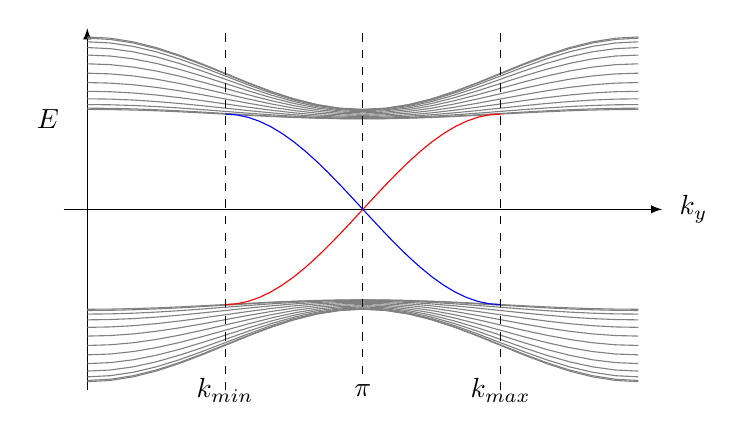
\begin{tikzpicture}

\def \vsize{2.3}
\def \hsize{7}
\def \u{1.3}

\draw [-latex] (0,-\vsize) -- (0,\vsize);
\draw [-latex] (-0.3cm,0) -- (\hsize+0.3,0);

\draw node at (-0.5cm,0.5*\vsize) {$E$};
\draw node at (\hsize cm + 0.7cm, 0) {$k_y$};

\def\bandsteps{12}

\foreach \n in {0, ...,\bandsteps }
{	
	\draw [domain = 0:\hsize, variable= \x, gray] plot ({\x cm},{ 1.1+0.1*(sin(\x*360/\hsize)*sin(\x*360/\hsize) + sin(\n*180/\bandsteps)*sin(\n*180/\bandsteps) + (\u + cos(\x*360/\hsize)  +cos(\n*180/\bandsteps) )*(\u + cos(\x*360/\hsize)  +cos(\n*180/\bandsteps) )  ) });
	\draw [domain = 0:\hsize, variable= \x, gray] plot ({\x cm},{ -1.1-0.1*(sin(\x*360/\hsize)*sin(\x*360/\hsize) + sin(\n*180/\bandsteps)*sin(\n*180/\bandsteps) + (\u + cos(\x*360/\hsize)  +cos(\n*180/\bandsteps) )*(\u + cos(\x*360/\hsize)  +cos(\n*180/\bandsteps) )  ) });
}

\def\scale{1.21}
\draw [domain = -0.25*\hsize:0.25*\hsize, variable= \x, red] plot ({\x +0.5*\hsize},{ \scale*sin(\x*360/\hsize) });
\draw [domain = -0.25*\hsize:0.25*\hsize, variable= \x, blue] plot ({\x +0.5*\hsize},{ -\scale*sin(\x*360/\hsize) });

\draw [dashed] (0.25*\hsize,-\vsize) -- (0.25*\hsize,\vsize);
\draw [dashed] (0.75*\hsize,-\vsize) -- (0.75*\hsize,\vsize);
\draw [dashed] (0.5*\hsize,-\vsize) -- (0.5*\hsize,\vsize);
\draw node [] at (0.25*\hsize,-\vsize) {$k_{min}$};
\draw node [] at (0.75*\hsize,-\vsize) {$k_{max}$};
\draw node [fill=white] at (0.5*\hsize,-\vsize) {$\pi$};
\end{tikzpicture}
\end{center}
\begin{center}
\begin{tabular}{ r l }
 $k_y \in (0, k_{min})$ : & $P_{k_y}$ contains $L_x$ bulk states \\ 
 $k_y \in (k_{min},\pi)$ : & $P_{k_y}$ contains $L_x -1 $ bulk states and one right-edge state  \\  
  $k_y =\pi $ : & $P_{k_y}$ contains $L_x -1 $ bulk states and both edge states  \\  
 $k_y \in (\pi, k_{max})$ : & $P_{k_y}$ contains $L_x -1 $ bulk states and one left-edge state  \\ 
 $k_y \in ( k_{max} , 2\pi)$ : & $P_{k_y}$ contains $L_x$ bulk states
\end{tabular}
\end{center}
At $k_{min}$ and $k_{max}$, a bulk state smoothly transitions into an edge state and vice-versa, so the change in $P_{k_y}$ is continuous. However at $k_y = \pi$, a right-edge state vanishes and a left-edge state appears, causing $P_{k_y}$ to change discontinuously. These states are able to suddenly disappear and appear because they cross the Fermi level, which is assumed to be a hard cutoff. As we will see, this discontinuity is the source of all of our troubles.\par
To understand where this causes problems we will expand the expression in eqn. \ref{eqn:strip_bott_index} to first order in $\delta_x$. This is reasonable since we are already working under the assumption that $L_x$ is large. We look only at the operator that appears in the logarithm, which we label $\hat M_{k_y}$,
\begin{align}
	\hat M_{k_y} &= \hat P_{k_y}  e^{i \delta_x \hat x}  \hat P_{k_y} \hat P_{k_y - \delta_y} e^{-i \delta_x \hat x}  \hat P_{k_y - \delta_y} \hat P_{k_y} + \hat Q_{k_y} \\
	\begin{split}\label{eqn:m_taylor}
		& = \hat P_{k_y} \hat P_{k_y - \delta_y} \hat P_{k_y} + \hat Q_{k_y} \\
		&\phantom{=}\, + i \delta_x \hat P_{k_y} \left ( \hat X_{k_y} - \hat X_{k_y- \delta_y }  \right )\hat P_{k_y - \delta_y} \hat P_{k_y}
	+ O(\delta_x^2).
	\end{split}
\end{align}
Now suppose that we are looking at a particular value of $k_y$ such that $k_y - \delta_y < \pi < k_y$, furthermore we will assume that  $\delta_y$ is extremely small, ensuring that the energy eigenstates themselves do not change significantly between $k_y - \delta_y $ and $ k_y$. This means that $P_{k_y}$ contains a left-edge state and $P_{k_y-\delta_y}$ contains a right-edge state. Thus the operator $\hat P_{k_y} \hat P_{k_y - \delta_y} \hat P_{k_y}$ only contains bulk states\footnote{This is not quite true, the states themselves change slightly with $k_y$, so this statement is approximate rather than exact. However as the value of $\delta_y$ gets smaller this statement gets closer and closer to being exact.}. $\hat Q_{k_y}$ will only contain a right-edge state, so the combination $ \hat P_{k_y} \hat P_{k_y - \delta_y} \hat P_{k_y} + \hat Q_{k_y} $ looks like the identity but with a single missing eigenvalue -- where the missing left-edge state is. This will occur whenever $k_y$ and $k_y - \delta_y$ sit on opposite sides of a point where the edge states cross the Fermi level.\par
This causes problems in our calculations. As we see in expression \ref{eqn:m_taylor}, $\hat M_{k_y}$ looks like it should have the form $\hat M_{k_y} = \1 + W_{\textup{small}}$, where $W$ is just some operator with eigenvalues $\ll 1$. This would mean that $\log \hat M_{k_y} \approx W_{\textup{small}}$.  However for certain values of $k_y$, the the operator $ \hat P_{k_y} \hat P_{k_y - \delta_y} \hat P_{k_y} + \hat Q_{k_y}$ is almost the identity but with one very small eigenvalue. When we take a log of the operator, this missing eigenvalue gives a huge contribution, since the log diverges at zero. \par
Now we can see where the strange edge behaviour of the Bott index comes from. This tiny eigenvalue of $\hat M_{k_y}$ has as its eigenvector the missing state from $ \hat P_{k_y} \hat P_{k_y - \delta_y} \hat P_{k_y} + \hat Q_{k_y} $. This missing state is always an edge state, so effect is to create a large distortion to the Bott index that lives on the support of that edge state. This is precisely what we see when we calculate the Bott index in strip geometry, as shown in fig. \ref{fig:edge_bott}.
\begin{figure}[t]
\begin{center}
 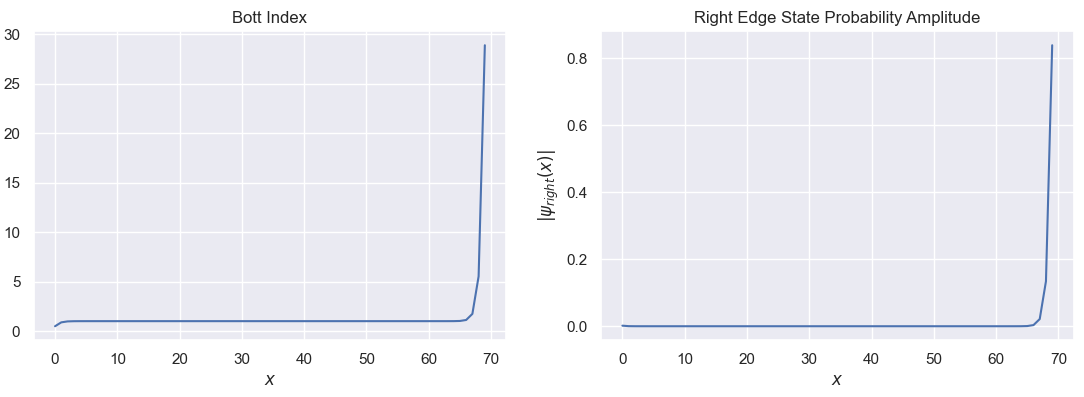
\includegraphics[width=0.8\textwidth]{edge_bott}
\caption{Strip Bott index calculated for a material with $L_x  = L_y = 70$, $u = 1.4$ compared to the probability distribution of the right edge state. A large discontinuity can be seen on the right hand side of the Bott index that closely matches the shape of the right edge state, supporting our assertion that the edge behaviour of the Bott index is due to a term in the sum that lives on the support of one edge state.}
\label{fig:edge_bott}
\end{center}
\end{figure}

\subsubsection{Generalising the Argument}
We can now give a looser and more general understanding for why these problems are appearing in our calculations. When we calculate the Chern number of a band, what we essentially want to do is take every state in that band, and push it adiabatically around a plaquette in $k$-space. We look at the phase that each state accumulates, and sum them to get $\mathcal Q$.

\begin{center}
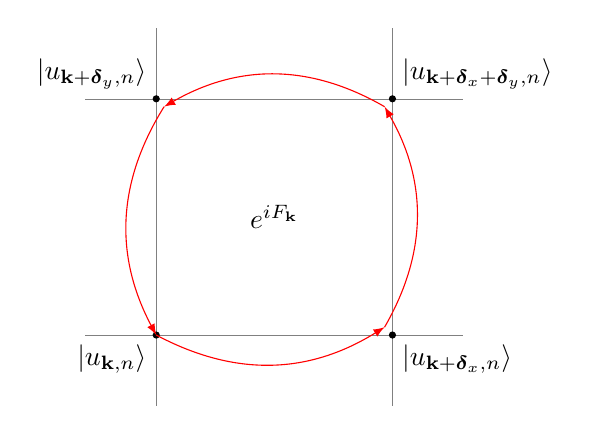
\begin{tikzpicture}

\def \gridsize{3}
\def \in {0.4}
\def\lineoffset{0.1}

\draw[step=\gridsize cm, help lines] (-0.3*\gridsize,-0.3*\gridsize) grid (1.3*\gridsize,1.3*\gridsize);

 
\foreach \x in {0, ..., 1}{
\foreach \y in {0, ..., 1}{
\fill[] (\x*\gridsize , \y*\gridsize) circle (1.3pt);
}}

\draw [red , -latex] (0,0) to [bend right] (\gridsize-\lineoffset,0+\lineoffset);
\draw [red , -latex] (\gridsize-\lineoffset,0+\lineoffset) to [bend right] (\gridsize-\lineoffset,\gridsize-\lineoffset);
\draw [red , -latex] (\gridsize-\lineoffset,\gridsize-\lineoffset) to [bend right] (0+\lineoffset,\gridsize-\lineoffset);
\draw [red , -latex] (0+\lineoffset,\gridsize-\lineoffset) to [bend right] (0,0);



 \draw node [fill= white] at ( 0.5*\gridsize, 0.5*\gridsize) {$e^{iF_{\bf k}}$};

\draw node [below left] at (0,0) {$\ket{u_{\bf k, n}}$};
\draw node [below right] at (\gridsize,0) {$\ket{u_{\bf k + \bm \delta_x, n}}$};
\draw node [above right] at (\gridsize,\gridsize) {$\ket{u_{\bf k + \bm \delta_x + \bm \delta_y , n}}$};
\draw node [above left] at (0,+\gridsize) {$\ket{u_{\bf k + \bm \delta_y, n}}$};

\end{tikzpicture}
\end{center}


However, this is not quite what happens when we calculate the Bott index! When we find the Bott index, what we are doing is using the $e^{i\delta_x \hat x}$ and $e^{i\delta_y \hat y}$ operators to shift the $\ket k$ part of each energy eigenstate, allowing us to take an inner product of adjacent states in $k$-space. We are looking at eigenstates that are adjacent to one another in $\hat P$ and expecting these to be closely adiabatically connected. When the system has no edge states -- no states cross the Fermi level -- this expectation proves to be correct, so the calculation is equivalent to pushing one state around a loop.
\begin{center}
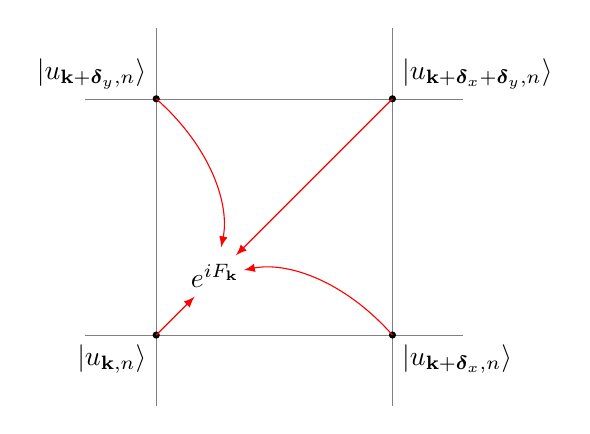
\begin{tikzpicture}

\def \gridsize{3}
\def \in {0.4}
\def\labeloffset{0.5}

\draw[step=\gridsize cm, help lines] (-0.3*\gridsize,-0.3*\gridsize) grid (1.3*\gridsize,1.3*\gridsize);

 
\foreach \x in {0, ..., 1}{
\foreach \y in {0, ..., 1}{
\fill[] (\x*\gridsize , \y*\gridsize) circle (1.3pt);
}}

 \draw node [fill= white] at ( 0.25*\gridsize, 0.25*\gridsize) {$e^{iF_{\bf k}}$};

\draw [red,-latex,shorten >=0.37cm ] (\gridsize,0) to [bend right] (0.25*\gridsize, 0.25*\gridsize);
\draw [red , -latex,shorten >=0.37cm] (\gridsize,\gridsize) to [] (0.25*\gridsize, 0.25*\gridsize);
\draw [red, -latex,shorten >=0.37cm] (0,\gridsize) to [bend left] (0.25*\gridsize, 0.25*\gridsize);
\draw [red, -latex,shorten >=0.37cm] (0,0) to [] (0.25*\gridsize, 0.25*\gridsize);



\draw node [below left] at (0,0) {$\ket{u_{\bf k, n}}$};
\draw node [below right] at (\gridsize,0) {$\ket{u_{\bf k + \bm \delta_x, n}}$};
\draw node [above right] at (\gridsize,\gridsize) {$\ket{u_{\bf k + \bm \delta_x + \bm \delta_y , n}}$};
\draw node [above left] at (0,+\gridsize) {$\ket{u_{\bf k + \bm \delta_y, n}}$};

\end{tikzpicture}
\end{center}
However when a state crosses the Fermi level, this allows the states in $\hat P$ to change discontinuously as you try to translate $\hat P$ in $k$-space. That means when you are comparing states that are adjacent to one another, you end up inadvertently comparing states on either side of some discontinuous jump in $\hat P$. This is exactly what happened in \textsection\ref{sec:discontinuities_example}, where we ended up trying to take a product between a left edge state and a right edge state. Since these states are not closely related to one another, we cannot expect to get a reasonable number for the relative phase between them, and our calculation breaks down.\par
Now that we have a sense of what is going wrong, we can try to construct a definition of the Bott index that does not suffer from these issues. Central to this will be the idea of trying to build a Bott index using operators that translate us adiabatically through $k$-space.

\subsection{Adiabatic Bott Index}

We now try and invent something that looks like a Bott index, but relies only on adiabatic translations through $k$-space, as hopefully this will allow us to avoid hitting discontinuities in our projector. This work is unfinished, here we will lay some of the groundwork and explain the central idea, however it is currently unclear whether this method will produce the desired result. Central to this is the notion of adiabatic flux insertion, a technique that has been used to understand fractionalisation in quantum many body systems \cite{oshikawa_fractionalization_2006}. We start by looking at how to include the presence of a magnetic field in a lattice system -- using Peierls substitution. We can then use this to construct a set of operators representing the slow insertion of magnetic flux through our system. Hopefully these should provide a pathway to constructing $k$-translation operators with which to define a stabilised Bott index.

\subsubsection{Peierls Substitution}

We first introduce an approximate technique to describe the effect of a slowly-varying magnetic field on a tight-binding quantum system first introduced in \cite{peierls_zur_1933}, although a description in English can be found in \cite{hofstadter_energy_1976}. The Peierls substitution states that in the presence of a magnetic vector potential $\bf A$, the translation operators that form the Hamiltonian change according to
\begin{align}
	\hat T_x \rightarrow \ket{\bf m + 1_x}\bra{\bf m} e^{i \theta_{\bf m}^x}, \ \hat T_y \rightarrow \ket{\bf m + 1_y}\bra{\bf m} e^{i \theta_{\bf m}^y},
\end{align}
where $\theta$ is just the line integral of the vector potential between two adjacent sites on the lattice,
\begin{align}
	\theta_{\bf m}^x = \frac{q}{\hbar}\int_{\bf m}^{\bf m + 1_x} \bf A(\bf r) \cdot d\bf r, \ \theta_{\bf m}^y = \frac{q}{\hbar}\int_{\bf m}^{\bf m + 1_y} \bf A(\bf r) \cdot d\bf r.
\end{align}\par
Now suppose that we have some material on a two dimensional square lattice and we introduce a uniform potential $\bf A$ across the whole material. If the lattice points are equally spaced apart, this will mean that every nearest-neighbour translation operator picks up a constant phase $\theta_x$ or $\theta_y$, and each longer-range operator picks up a phase proportional to the distance in each direction. Thus a Hamiltonian in such a system given by
\begin{align}
	\hat H  = \sum_{\bf m, \bf n} \ket{\bf m} \bra{\bf n} \otimes \hat H^{int}_{\bf m, \bf n}
\end{align}
is modified to
\begin{align}
	\hat H(\bf A)  = \sum_{\bf m, \bf n} \ket{\bf m} \bra{\bf n} e^{i \theta_x(m_x - n_x) + \theta_y(m_y - n_y)} \otimes \hat H^{int}_{\bf m, \bf n}.
\end{align}
This is exactly equivalent to making the following transformation
\begin{align}
	\hat H \rightarrow \hat H (\bf A) = e^{i \bm \theta \cdot \hat{ \bf x}} \hat H e^{-i \bm \theta \cdot  \hat{ \bf x}},
\end{align}
so we realise that we have already been working with these kinds of transformations already, and know exactly their effect -- to translate our states around $k$-space by the vector $\bm \theta$!

\begin{shaded}
	Something weird is going on -- for values of $\theta \neq \frac{2\pi p}{L_x}$ where $p$ is an integer, the exponential operator here is not periodic with the system and so isn't well-defined! It turns out this does not matter, since the operator is only used to add a phase to the off-diagonal elements of $\hat H$.
\end{shaded}

\subsubsection{Adiabatic Flux Insertion}

The idea here is that we can use the slow insertion of magnetic flux to transport our states around the Brillouin zone. We define a pair of operators $\hat{\mathcal{F}}_x$ and $\hat{\mathcal{F}}_y$ that represent the gradual ramping up of a magnetic vector potential in either the $x$ or the $y$-direction. This is ramped up from $A = 0$ to 
\begin{align}
	A_x = \frac{2\pi\hbar}{q \Delta_x L_x},
\end{align}
where $\Delta_x$ is the distance between unit cells in the lattice. We use the equivalent expression for $\hat{\mathcal F}_y$. These values are chosen such that at the end $\theta_x = \frac{2\pi}{L_x}$ and $\theta_y = \frac{2\pi}{L_y}$. When acted on a state $\ket{\psi_{\bf k, n}}$, the operator $\hat{\mathcal{F}}_x$ should be able to transform it to $\ket{\psi_{\bf k + \delta_x, n}}$. Since it is adiabatic it will not mix between states  at different energy. Furthermore, the operator is local, and this should ensure that in a large system it is prohibited from mixing between a left edge state and a right edge state.\par
Thus we can use these operators in place of $e^{i \delta_x \hat x}$ and $e^{i \delta_y \hat y}$ in the definition of the Bott index. These have the advantage that when acted on a projector containing bulk states and one left edge state, for example, they will only be able to map it to a new projector containing the same types of states, but translated in $k$-space. This allows us to avoid the discontinuities encountered in \textsection\ref{sec:discontinuities_example}. In the case where there are no states crossing the Fermi level and $\hat P_{k_y}$ is continuous it should be exactly identical to the standard definition of Bott index.



\section{Conclusions and Outlook}
%!TEX root = ./main.tex

In this document we have looked at the properties of topological insulators, focussing on the example of the QWZ model -- a simple tight binding model with nearest neighbour interactions. We have introduced the definition of the Berry phase, Berry connection and Chern number, and seen how these can be used to classify the Hamiltonians of translationally symmetric quantum systems, as well understanding their role in the formation of gapless edge modes. Furthermore we have discussed the limitations of these concepts -- that they are only applicable to systems with periodic boundaries and translational symmetry. We introduce two efforts to extend the notion of Chern number to systems that do not fulfil these criteria, namely the Bott index and Chern number, and show how they are related. These quantities display some strange behaviour, such as being discontinuous where boundaries appear in the material, or showing some global rather than local properties. We have worked towards better understanding the causes of these discontinuities, as well as trying to understand whether they convey useful physical information. \par
Finally, we have introduced a set of tools that we hope will allow us to modify the definition of the Bott index to avoid the discontinuous behaviour at the edges. The modifications are based on the application of slowly varying magnetic flux to the material. This remains unfinished and it is not yet clear whether they will prove as useful as we hope. Many questions remain, firstly it is unclear whether adiabatic flux insertion is capable of providing us with stable operators that effect translation in $k$-space. Especially since any finite system will have some degree of coupling between opposing edge modes, allowing a left edge mode to transform into a right edge mode as $k$ is varied. It is not yet clear whether this will provide a significant obstacle to the creation of adiabatic operators that preserve left and right edge states. Furthermore the exact form of operators representing adiabatic flux insertion have not yet been calculated and tested to ensure that they have the right properties. In the short term the author intends to find the exact form of these operators and numerically test that they have the right properties and that an adiabatic Bott index using them is stable. This will be followed by efforts to write an analytic proof demonstrating the validity of this method. If this works, next steps will be to determine whether this stabilised Bott index has a physically significant interpretation. One candidate for this is to check wither it corresponds to a local definition of electric polarisation, since our current understanding of polarisation views it as a global quantity \cite{vanderbilt_berry_2018} -- in contrast to the classical picture. \par
In the longer term we have several further avenues to explore. One possibility is to examine whether these concepts can be used to determine the topological properties of interacting systems. It is not clear whether it is possible to create an equivalent Bott index that can act on a many-particle interacting ground state. Another possible avenue is to look at the behaviour of the Bott index in a system evolving dynamically. The author has found that the standard Bott index is unstable when applied to a quenched system similar to that used in \cite{caio_topological_2019}, so an interesting question could be to understand where this instability comes from and test whether it can be controlled by modifying the Bott index.
\small
\bibliography{early_stage_review.bib}
\normalsize
%!TEX root = ./main.tex
\newpage

\appendix

\section{Proof of Bloch's Theorem}\label{appendix:bloch_proof}
Bloch's theorem states that any Hamiltonian with crystalline periodic symmetry, where the particles move in a periodic potential, $V(\bf x)$ with
\begin{align}
    V(\bf x + \bf R) = V(\bf x),
\end{align}
must have eigenstates of the form
\begin{align}
    \psi_{n,\bf{k}}(\bf{x} )  = e^{i\bf{k}\cdot \hat{\bf{x}}}  u_{n,\bf{k}}(\bf{x} ) ,
\end{align}
where $\bf k$ is a wave vector that lies in the first Brioullin zone and the state $u_{n,\bf{k}}(\bf{x} )$ is periodic on the unit cell. \par
Let's prove this. Since $V$ is periodic, it may be written as a sum of discrete Fourier components.
\begin{align}
    V(\bf{x}) = \sum_{\bf{G}} V_{\bf{G}} e^{i \bf{G} \cdot \bf{x}},
\end{align}
where the sum is over reciprocal lattice vectors. Now, writing the states $\psi$ in the Fourier basis
\begin{equation}
    \psi(\bf{x}) = \frac{1}{(2\pi)^n} \int d\bf{q}\ \tilde{\psi}(\bf{q})\ e^{i \bf{x}\cdot \bf{q}},
\end{equation}
we may rewrite the Schr\"{o}dinger equation as
\begin{equation}
    \int d\bf{q}\ \left ( \frac{\hbar^2 \bf{q}^2}{2m}- E + \sum_\bf{G}V_{\bf{G}} e^{i \bf{G} \cdot \bf{x}} \right )\tilde{\psi}(\bf{q})\ e^{i \bf{x}\cdot \bf{q}} = 0 .
\end{equation}
Now we can rewrite the second term on the LHS as
\begin{align}
    \int d\bf{q}\ \sum_\bf{G} V_\bf{G} e^{i\bf{G}\cdot\bf{x}} \tilde{\psi}(\bf{q})\ e^{i \bf{x}\cdot \bf{q}} = \int d\bf{q}\ \sum_\bf{G} V_\bf{G} \tilde{\psi}(\bf{q}-\bf{G})\ e^{i \bf{x}\cdot \bf{q}},
\end{align}
since the integral is over all possible values of $\bf{q}$. Thus, we get
\begin{equation}
    \int d\bf{q}\ \left [ \left ( \frac{\hbar^2 \bf{q}^2}{2m}- E  \right )\tilde{\psi}(\bf{q}) + \sum_\bf{G}V_{\bf{G}} \tilde{\psi}(\bf{q}-\bf{G})\ \right ] e^{i \bf{x}\cdot \bf{q}} = 0 .
\end{equation}
The term inside the bracket no longer has any more $\bf{x}$-dependence! This means that the condition must hold independently for all values of $\bf{q}$ in the integral. Thus we get the relation
\begin{equation}\label{eqn:k_schrodinger}
    \left ( \frac{\hbar^2 \bf{q}^2}{2m}- E  \right )\tilde{\psi}(\bf{q}) + \sum_\bf{G}V_{\bf{G}} \tilde{\psi}(\bf{q}-\bf{G})\ = 0 .
\end{equation}
What is happening here? We have almost managed to decouple the equations for $\psi(\bf{q})$ for different values of $\bf{q}$. We've been left with an expression that couples each $\psi(\bf{q})$ with all of the expressions that differ from it by a reciprocal lattice vector. This means that the coefficients of $\psi$ in the Brillouin zone are fully decoupled, but each comes with an infinite series of higher Fourier coefficients that are spaced out with the reciprocal lattice. Thus, for every value of $\bf{k}$ in the Brillouin zone, we can create a state $\psi_\bf{k}(\bf{x})$ that may be written as
\begin{align}
    \psi_\bf{k}(\bf{x}) = \sum_{G} C_\bf{G} e^{i\bf{x} \cdot (\bf{k}+\bf{G})}.
\end{align}
Pulling the $\bf{k}$ term out of the sum we get our final result
\begin{align}
    \psi_{\bf{k},n}(\bf{x}) &= e^{i \bf{k} \cdot \bf{x}}\sum_{G} C_\bf{G} e^{i\bf{x} \cdot \bf{G}}  \\
    &=e^{i \bf{k} \cdot \bf{x}}\ u_{\bf{k},n}(\bf{x}),
\end{align}
where the $n$ subscript references the fact that equation \ref{eqn:k_schrodinger} may have multiple solutions, each denoting a different band in the material.\par
Why should we expect $\bf{k}$ to live inside the first Brillouin zone? This is because if $\bf{k}$ is outside the Brillouin zone, then we can write $\bf{k} = \bm{\kappa} + \bf{G}$ where $\bm{\kappa}$ is in the first Brillouin zone and $\bf{G}$ is a reciprocal lattice vector. now our expression for $\psi$ becomes
\begin{align}
    \psi_{\bf{k},n}(\bf{x}) =e^{i \bm{\kappa} \cdot \bf{x}}e^{i \bf{G} \cdot \bf{x}}\ u_{\bf{k},n}(\bf{x}).
\end{align}
Here, $e^{i \bf{G} \cdot \bf{x}}$ is also periodic in the unit cell, so we can just incorporate it into the expression for $u_{\bf{k},n}(\bf{x})$.

\section{Direct Calculation of Berry Curvature for a Two Level System} \label{sec:berry_curvature_two_level}

We are tasked with finding the Berry curvature for the eigenstates of a general $2 \times 2 $ Hamiltonian, parametrised by a vector $\bf d$ in $\mathbb R^3$ according to
\begin{align}
    H = |\textbf{d}|\begin{pmatrix}
\cos(\theta) &e^{-i\phi}\sin{\theta} \\ 
 e^{i\phi}\sin{\theta}& -\cos(\theta)
\end{pmatrix},
\end{align}
Where the vector is expressed in spherical polar coordinates. This Hamiltonian has positive and negative eigenstates with energy $\pm |\bf d |$ and wavefunctions
\begin{align}
    \ket{+_{\textbf{d}}} = \begin{pmatrix}
e^{-i\phi/2}\cos(\theta/2)\\ 
e^{i\phi/2} \sin(\theta/2)
\end{pmatrix},\; \ket{-_{\textbf{d}}} = \begin{pmatrix}
-e^{-i\phi/2}\sin(\theta/2)\\ 
e^{i\phi/2} \cos(\theta/2)
\end{pmatrix}.
\end{align}
We wish to find the Berry connection and curvature, given by
\begin{align}
    \textbf{A}^\pm (\bf d) &= i\braket{\pm_\textbf{d} | \nabla_\textbf{d}| \pm_\textbf{d}}\\
    \textbf{B}^{\pm}(\bf d ) &= \nabla_\textbf{d} \wedge \textbf{A}^\pm (\bf d).
\end{align}
From here it is possible to directly evaluate the Berry curvature of the two eigenstates, however there is an easier way of doing this, using a trick first proposed by Berry in \cite{berry_quantal_1984}. First we note that $ \nabla_\textbf{d} \braket{\pm_\textbf{d} | \pm_\textbf{d}} = 0$, due to invariance of the norm. Thus we can show that $\braket{\pm_\textbf{d} | \nabla_\textbf{d}| \pm_\textbf{d}}$ is pure imaginary. Expressing this in terms of a general state $\ket{n}$ ,
\begin{align}
    \textbf{A} (d) &= -\textup{Im} \braket{n | \nabla| n}.
\end{align}
Now, in summation notation our expression for $\textbf{B}$ is
\begin{align}
    B_j &= -\textup{Im}\;\epsilon_{jkl}\,\partial_k\, \braket{n | \partial_l| n}\\
    &=-\textup{Im}\; \epsilon_{jkl}\braket{\partial_k n|\partial_l n}
\end{align}
We then insert a resolution of the identity to get
\begin{align}
    \textbf{B} = -\textup{Im}\;\sum_{n'\neq n}\braket{\nabla n|n'}\wedge\braket{n'|\nabla n}
\end{align}
For two general orthogonal states $\ket{n}$ and $\ket{n'}$
\begin{align}
    \nabla (\hat H \ket{m}) &= \nabla (E_n \ket{n})\\
    \nabla \hat H \ket{m}+\hat  H\ket{\nabla n} &= \nabla E_n \ket{n}+ E_n\ket{\nabla n} .
\end{align}
Pre-multiplying by $\bra{n'}$ gives
\begin{align}
\braket{n'|\nabla\hat  H|n} + E_{n'}\braket{n'|\nabla n} = E_n\braket{n' | \nabla n},
\end{align}
therefore
\begin{align}
    \braket{n'|\nabla n} = \frac{\braket{n'|\nabla\hat  H|n}}{E_n - E_{n'}}.
\end{align}
And so we get a final expression for $\bf B$
\begin{align}\label{berry_formula}
\textbf{B} = -\textup{Im}\;\sum_{n'\neq n} \frac{\braket{n|\nabla\hat  H|n'} \wedge \braket{n'|\nabla\hat  H|n}}{(E_n - E_{n'})^2}.
\end{align}
From this we can see that the Berry curvature of the $\ket{+_\textup{d}}$ state is given by
\begin{align}
    \textup{B} = -\textup{Im}\; \frac{\braket{+|\nabla H|-} \wedge \braket{-|\nabla H|+}}{4\textbf{d}^2}.
\end{align}
To simplify the calculations we will quantise in a basis of states parallel to $\textbf{d}$. Thus, our states are
\begin{align}
    \ket{+_{\textbf{d}}} = \begin{pmatrix}
1\\ 
0
\end{pmatrix},\; \ket{-_{\textbf{d}}} = \begin{pmatrix}
0\\ 
1
\end{pmatrix}.
\end{align}
The grad of the Hamiltonian is
\begin{align}
    \nabla_\textbf{d} (\textbf{d} \cdot \hat{\sigma} )= \hat{\sigma}
\end{align}

\begin{shaded}
Quick point of confusion, just in case you were wondering why we could simplify the calculation so much without losing information. All we have done is pick a basis in which to express our states and Hamiltonian such that the calculation at that particular point in d-space is trivial. If you want to know what the value of $\textbf{B}$ is in a different place, then you can just rotate the coordinates again to get them parallel with $\textbf{d}$ and again you get an identical calculation. This might seem kind of obvious, but I had to think about it.
\end{shaded}
Now we find the values of $\braket{-|\sigma_j | +}$:
\begin{align}
    \braket{-|\sigma_x | +} &= 1 \\
    \braket{-|\sigma_y | +} &= i \\
    \braket{-|\sigma_z | +} &= 0 \\
\end{align}
And we arrive at 
\begin{equation}
    \braket{+|\hat{\sigma} | -} \wedge \braket{-|\hat{\sigma} | +} = \begin{pmatrix}
    0 \\
    0 \\
    2i
    \end{pmatrix}
\end{equation}
The Berry curvature always points outwards from the origin in d-space, thus we arrive at the final expression
\begin{align}
    \textbf{B}^{\pm} = \pm \frac{\hat{n}_\textbf{d}}{2\textbf{d}^2}
\end{align}
where $\hat{n}_\textbf{d}$ is a unit vector pointing in the direction of $\textbf{d}$.\par

\section{Eigenstates of the QWZ Model}\label{sec:QWZ_model_appendix}

We are looking for the solutions to the semi-bulk Hamiltonian
\begin{align}
    H(k_y) &= \sum_{m_x} \ket{m_x+1}\bra{m_x} \otimes \frac{\sigma_z + i\sigma_x}{2} + h.c.\nonumber \\
    &+ \sum_{m_x} \ket{m_x}\bra{m_x} \otimes \left [ (u_{m_x} + \cos k_y) \; \sigma_z + \sin k_y \; \sigma_y  \right ].
\end{align}
From here on in, we will only be able to use Bloch's theorem in the $y$ direction, so we drop $y$ subscripts on $k_y$. We look at a system where the Hamiltonian has open boundaries in $x$ and uniform $u$ throughout. For clarity we display the Hamiltonian in the following form
\begin{align}
    H(k_y) = \begin{pmatrix}
 A& B &  &  & &\\ 
 B^\dag& A &B  &  & &\\ 
 &  B^\dag& A &  \ddots& &\\ 
 &  &  \ddots& \ddots & &\\ 
 &  &  & & &B\\
 &  & & & B^\dag & A
\end{pmatrix},
\end{align}
with $A$ and $B$ being the $2\times2$ matrices
\begin{align}
    A &= (u + \cos k) \; \sigma_z + \sin k \; \sigma_y,  \\ 
    B &= \frac{\sigma_z + i\sigma_x}{2}.
\end{align}
By writing wavevectors in terms of a set of $L_x$ two-element states $\psi_n$
\begin{align}
    \ket{\psi} = \begin{pmatrix}
    \psi_0 \\
    \psi_1 \\
    \vdots \\
    \psi_{L_x -1}
     \end{pmatrix},
\end{align}
we arrive at three equations for the eigenvalues of the semi-bulk Hamiltonian.
\begin{align}
    \textup{Bulk:} &\ A\psi_n + B\psi_{n+1} + B^\dag \psi_{n-1} = \lambda \psi_n \\
    \textup{Left Edge:} &\ A\psi_1 + B\psi_{2} = \lambda \psi_1\\
    \textup{Right Edge:} &\ A\psi_{L_x} + B^\dag \psi_{L_x-1}  = \lambda \psi_n
\end{align}
An equivalent way of writing the two edge conditions above is to say that we require
\begin{align}
    B^\dag \psi_{0} &= 0\\
    B \psi_{L_x+1} &= 0.
\end{align}
Solutions to this equation fall into two categories, bulk states and edge states. We will solve for each separately.\par
Before we continue, it is a good idea to change the basis we are using to make the form of the $B$ matrix simpler. This matrix is essentially a creation/annihilation operator, so there should be a basis in which the matrix has the form
\begin{align}
    \tilde{B} = \begin{pmatrix}
    0 & 1 \\
    0 & 0 
     \end{pmatrix}.
\end{align}
This can be done using the unitary transformation operator
\begin{align}
    U = \frac{1}{\sqrt{2}}\begin{pmatrix}
    1 & 1 \\
    i & -i 
     \end{pmatrix}.
\end{align}
Using this expression for $U$ we have 
\begin{align}
    \tilde B  = U^\dag B U 
\end{align}
and 
\begin{align}
    \tilde A &= U^\dag A U \\
    &= (u + \cos k) \; \sigma_x + \sin k \; \sigma_z.
\end{align}
In the following work we will replace all $A$s and $B$s with $\tilde A$ and $\tilde B$ and drop the tilde. 

\subsection{Bulk States}
With this established, we can now solve the bulk equation for its eigenstates using the following ansatz
\begin{align}
    \psi_n = e^{i\theta n}\phi_{\theta},
\end{align}
with $0 \leq \theta < \pi$. Plugging this into the bulk equation we arrive at
\begin{align}
    A\phi_{\theta} + Be^{i\theta}\phi_{\theta} + B^\dag e^{-i\theta} \phi_{\theta} = \lambda \phi_{\theta}
\end{align}
which can be rearranged to the following bulk Hamiltonian,
\begin{align}
    H(\theta, k) = \begin{pmatrix}
 u + \cos \theta+ \cos k \\ 
- \sin \theta\\ 
 \sin k
\end{pmatrix} \cdot \bm \sigma.
\end{align}
The eigenvalues of this matrix are
\begin{align}
    \lambda_{\pm} = \pm E,
\end{align}
for
\begin{align}
    E = \left [ \sin^2 k + \sin^2 \theta  + \left ( u + \cos \theta+ \cos k \right)^2 \right ]^{\frac{1}{2}}.
\end{align}
It has (unnormalised) eigenvectors
\begin{align}\label{eigenvectors}
    \phi_+ &= \begin{pmatrix}
\sin k + E\\
u + \cos k + e^{-i\theta}
\end{pmatrix}\\ 
    \phi_- &=\begin{pmatrix}
-u -  \cos k - e^{i\theta}\\
\sin k + E
\end{pmatrix}
\end{align}
We could normalise these if we wanted to, but it gets messy, instead we notice that the eigenvalues of a Hamiltonian of the form $H = \bf n \cdot \bm \sigma$ are always $E = \pm |\bf n |$. This is useful, it means that for a given $\theta$ we have a pair of states $ \phi_\theta ^\pm$ with energy $\pm E_\theta$. However, looking at the expression for $E$ we see that $E_\theta = E_{-\theta}$. Since these states have the same energy, we can use them to construct standing-wave solutions according to
\begin{align}
    \ket{\psi^\pm_{|\theta|} }= \frac{1}{\sqrt{L_x}}\sum \ket{m}  \otimes \left [ \alpha e^{i \theta m} \ket{\phi_{\theta}^{\pm}} + \beta e^{-i \theta m} \ket{\phi_{-\theta}^{\pm}} \right ],
\end{align}
with the condition $|\alpha|^2 + |\beta|^2=1$.\par
Before we continue let's notice one more thing. In $d$-space, we can see that $H(\theta, k) $ and $H(-\theta, k)$  are related by a reflection in the $y$-axis. This means that there exists an operator $\mathcal{S}$ that has the following property
\begin{align}
    \mathcal{S}^{-1} H(\theta,k)\mathcal{S}  = H(-\theta,k).
\end{align}
As it turns out, this operator is
\begin{align}
    \mathcal{S} = \mathcal{K},
\end{align}
Where $\mathcal{K}$ represents complex conjugation\footnote{$\mathcal{K}$ stands for komplexx, which is like complex but way cooler.}. This is pretty useful since you can show that if
\begin{align}
    H(\theta,k)\phi^\pm _{\theta} = \pm E_\theta \phi^\pm _{\theta}
\end{align}
then 
\begin{align}
    H(-\theta,k) \mathcal{S} \phi^\pm _{\theta} = \pm E_\theta \mathcal{S} \phi^\pm _{\theta},
\end{align}
which means that
\begin{align}
    {\phi^{\pm} _{\theta}}^*  = \phi^\pm _{-\theta}.
\end{align}
This gives us a straightforward transformation between the two states that we use to make up our ansatz for $\phi^\pm_{|\theta|}$. We have a final expression for $\psi_n$
\begin{align}
    \psi_{\theta,n} ^{\pm} = \alpha e^{i \theta m} \phi_{\theta}^{\pm} + \beta e^{-i \theta m} {\phi_{\theta}^{\pm}}^*.
\end{align}
For the following argument, lets assume that 
\begin{align}
    \phi_{\theta}^{\pm} = \begin{pmatrix}
    u \\ 
    v
    \end{pmatrix}.
\end{align}\par
Now we think about fixing the boundary conditions. We start with the left side boundary condition
\begin{align}
    B^\dag \psi_{0} &= 0.
\end{align}
Inserting our ansatz into this expression gives
\begin{align}
    \alpha u + \beta u^* = 0.
\end{align}
We then move on to the right side boundary condition
\begin{align}
    B \psi_{L_x + 1 } = 0,
\end{align}
and we insert our ansatz again to get
\begin{align}
    \alpha e^{i\theta (L_x + 1 )} v + \beta e^{-i\theta (L_x + 1 )} v^* = 0.
\end{align}
We can now solve these expressions to get
\begin{align}
    \frac{\beta}{\alpha} = - \frac{u}{u*} =  - e^{2i\theta (L_x + 1 )}\frac{v}{v*}.
\end{align}
Now we must look separately at $\phi^+$ and $\phi^-$, for $\phi^+$, $u$ is real in expression \ref{eigenvectors}, so the expression becomes
\begin{align}
    1 = e^{2i\theta (L_x + 1 )}\frac{u + \cos k + e^{-i\theta}}{u + \cos k + e^{i\theta}}.
\end{align}

\subsection{Edge States}
 For the edge states we return to our bulk and edge eigenvalue equations. However now we are looking at states that live only on one edge of the system. We will be looking at two edge states, one that lives on the left edge and one that lives on the right.\par
We rephrase the bulk and edge equations that need to be satisfied
\begin{align}
    \textup{Bulk:} &\ A\psi_n + B\psi_{n+1} + B^\dag \psi_{n-1} = \lambda \psi_n \\
    \textup{Left Edge:} &\ A\psi_1 + B\psi_{2} = \lambda \psi_1\\
    \textup{Right Edge:} &\ A\psi_{L_x} + B^\dag \psi_{L_x-1}  = \lambda \psi_n.
\end{align}
This time we guess an ansatz that looks like
\begin{align}
    \psi_n = \xi^n \phi,
\end{align}
where $\xi$ is a real number between -1 and 1. We are making the assumption that left side edge state will have decayed to nothing by the time it reaches the other side, we only need to satisfy the left edge boundary condition, and the same with the right edge state. This means we are working in the limit of a semi-infinite chain. Thus that we just need to guess a value of $\phi$ that satisfies 
\begin{align}
    B^\dag \phi = 0,
\end{align}
which has the solution
\begin{align}
    \phi_{\textup{left}} = \begin{pmatrix}
    0\\
    1
    \end{pmatrix}.
\end{align}
We now look at solving what's left of the bulk equation
\begin{align}
    (A + \xi B - \lambda)\phi_{\textup{left}} = 0,
\end{align}
to give the following two equations
\begin{align}
    \lambda &= -\sin k,\\
    \xi &= -u - \cos k.
\end{align}
Note that this solution only gives decaying results for $-1 < u+\cos k < 1$. Which corresponds with the window of $k$ values where edge states appear.
Thus we get a final wavefunction that looks like
\begin{align}
    \ket{\psi^{\textup{left}}_k} = \sqrt{1-\xi^2}\sum_{m=1}^{L_x} \xi^{m-1}\ket m \otimes \begin{pmatrix}
    0\\
    1
    \end{pmatrix}.
\end{align}
We can repeat the entire derivation for a right hand side wavefunction to get
\begin{align}
    \ket {\psi^{\textup{right}}_k} = \sqrt{1-\xi^2} \sum_{m=1}^{L_x} \xi^{L_x-m} \ket m \otimes  \begin{pmatrix}
    1\\
    0
    \end{pmatrix}.
\end{align}
with the extra conditions
\begin{align}
    \lambda &= \sin k,\\
    \xi &= -u-\cos k. \label{eqn:edge_condition}
\end{align}
Great.

\section{Taylor Expanding the Bott Index in Strip Geometry}\label{sec:bott_derivatives}
We want to Taylor expand the following operator,
\begin{align}
	\hat M_{k_y} &= \hat P_{k_y}  e^{i \delta_x \hat x}  \hat P_{k_y} \hat P_{k_y - \delta_y} e^{-i \delta_x \hat x}  \hat P_{k_y - \delta_y} \hat P_{k_y} + \hat Q_{k_y}.
\end{align}
This has the following set of derivatives in $\delta_x$ and $\delta_y$
\begin{align}
	\begin{split}
		\partial_{\delta_x} \hat M_{k_y} = 
		& i \hat P_{k_y} \hat x  e^{i \delta_x \hat x}  \hat P_{k_y} \hat P_{k_y - \delta_y} e^{-i \delta_x \hat x}  \hat P_{k_y - \delta_y} \hat P_{k_y} \\
		&-  i \hat P_{k_y}   e^{i \delta_x \hat x}  \hat P_{k_y} \hat P_{k_y - \delta_y} \hat x e^{-i \delta_x \hat x}  \hat P_{k_y - \delta_y} \hat P_{k_y},
	\end{split}\\
	\begin{split}
		\partial_{\delta_x}^2 \hat M_{k_y} = 
		& - \hat P_{k_y} \hat x^2  e^{i \delta_x \hat x}  \hat P_{k_y} \hat P_{k_y - \delta_y} e^{-i \delta_x \hat x}  \hat P_{k_y - \delta_y} \hat P_{k_y} \\
		&-   \hat P_{k_y}   e^{i \delta_x \hat x}  \hat P_{k_y} \hat P_{k_y - \delta_y} \hat x^2 e^{-i \delta_x \hat x}  \hat P_{k_y - \delta_y} \hat P_{k_y}\\
		&+ 2\hat P_{k_y} \hat x  e^{i \delta_x \hat x}  \hat P_{k_y} \hat P_{k_y - \delta_y} \hat x e^{-i \delta_x \hat x}  \hat P_{k_y - \delta_y} \hat P_{k_y} ,
	\end{split}\\
	\begin{split}
		\partial_{\delta_y} \hat M_{k_y} = 
		&  \hat P_{k_y} e^{i \delta_x \hat x}  \hat P_{k_y} \partial_{\delta_y} \hat P_{k_y - \delta_y} e^{-i \delta_x \hat x}  \hat P_{k_y - \delta_y} \hat P_{k_y}\\
		&+  \hat P_{k_y} e^{i \delta_x \hat x}  \hat P_{k_y}\hat P_{k_y - \delta_y} e^{-i \delta_x \hat x}  \partial_{\delta_y}  \hat P_{k_y - \delta_y} \hat P_{k_y},
	\end{split}\\
	\begin{split}
		\partial_{\delta_y}^2 \hat M_{k_y} = 
		&  \hat P_{k_y} e^{i \delta_x \hat x}  \hat P_{k_y} \partial_{\delta_y}^2 \hat P_{k_y - \delta_y} e^{-i \delta_x \hat x}  \hat P_{k_y - \delta_y} \hat P_{k_y}\\
		&+  \hat P_{k_y} e^{i \delta_x \hat x}  \hat P_{k_y}\hat P_{k_y - \delta_y} e^{-i \delta_x \hat x}  \partial_{\delta_y}^2  \hat P_{k_y - \delta_y} \hat P_{k_y}\\
		&+2  \hat P_{k_y} e^{i \delta_x \hat x}  \hat P_{k_y} \partial_{\delta_y} \hat P_{k_y - \delta_y} e^{-i \delta_x \hat x}  \partial_{\delta_y}  \hat P_{k_y - \delta_y} \hat P_{k_y},
	\end{split}
\end{align}
and finally
\begin{align}
	\begin{split}
		\partial_{\delta_x}\partial_{\delta_y} \hat M_{k_y} = 
		& i \hat P_{k_y} \hat x  e^{i \delta_x \hat x}  \hat P_{k_y}\partial_{\delta_y}  \hat P_{k_y - \delta_y} e^{-i \delta_x \hat x}  \hat P_{k_y - \delta_y} \hat P_{k_y} \\
		&+ i \hat P_{k_y} \hat x  e^{i \delta_x \hat x}  \hat P_{k_y} \hat P_{k_y - \delta_y} e^{-i \delta_x \hat x}  \partial_{\delta_y}\hat P_{k_y - \delta_y} \hat P_{k_y} \\
		&-  i \hat P_{k_y}   e^{i \delta_x \hat x}  \hat P_{k_y} \partial_{\delta_y}\hat P_{k_y - \delta_y} \hat x e^{-i \delta_x \hat x}  \hat P_{k_y - \delta_y} \hat P_{k_y}\\
		&-  i \hat P_{k_y}   e^{i \delta_x \hat x}  \hat P_{k_y} \hat P_{k_y - \delta_y} \hat x e^{-i \delta_x \hat x}  \partial_{\delta_y}\hat P_{k_y - \delta_y} \hat P_{k_y}.
	\end{split}
\end{align}
Awful. Now we set $\delta_x = \delta_y = 0 $ to get
\begin{align}
	\begin{split}
		\left . \partial_{\delta_x} \hat M_{k_y} \right |_{\delta_x , \delta_y = 0} &= 
		 i \hat P_{k_y} \hat x  \hat P_{k_y} -  i \hat P_{k_y}  \hat x\hat P_{k_y}\\
		& = 0,
	\end{split}\\
	\begin{split}
		\left . \partial_{\delta_x}^2 \hat M_{k_y} \right |_{\delta_x , \delta_y = 0} & = 
		 - 2\hat P_{k_y} \hat x^2   \hat P_{k_y} + 2\hat P_{k_y} \hat x  \hat P_{k_y} \hat x \hat P_{k_y} ,
	\end{split}\\
	\begin{split}
		\left . \partial_{\delta_y} \hat M_{k_y} \right |_{\delta_x , \delta_y = 0}& = 
		 -2\hat P_{k_y} \left ( \partial_{k_y} \hat P_{k_y} \right ) \hat P_{k_y},
	\end{split}\\
	\begin{split}
		\left . \partial_{\delta_y}^2 \hat M_{k_y} \right |_{\delta_x , \delta_y = 0}& = 
		 2 \hat P_{k_y} \left ( \partial_{k_y}^2 \hat P_{k_y}  \right ) \hat P_{k_y}
		+2  \hat P_{k_y}    \left ( \partial_{k_y} \hat P_{k_y } \right )^2 \hat P_{k_y},
	\end{split}\\
	\begin{split}
		\left . \partial_{\delta_x}\partial_{\delta_y} \hat M_{k_y} \right |_{\delta_x , \delta_y = 0}&= 
		-2 i \hat P_{k_y} \hat x \hat P_{k_y} \left ( \partial_{k_y}  \hat P_{k_y} \right)  \hat P_{k_y} \\
		&+  i   \hat P_{k_y} \partial_{k_y}\hat P_{k_y} \hat x  \hat P_{k_y } 
		+ i  \hat P_{k_y} \hat x  \partial_{k_y}\hat P_{k_y} \hat P_{k_y}.
	\end{split}
\end{align}
Thankfully we can also use the identity $\hat P_{k_y}  \left ( \partial_{k_y} \hat P_{k_y} \right ) \hat P_{k_y} = 0$ to throw away some of these terms and we label the projected $x$ operator $\hat X_{k_y} = \hat P_{k_y} \hat x  \hat P_{k_y}$. We arrive at the following Taylor expansion
\begin{align}
	\begin{split}
		\hat M_{k_y}  &= \hat P_{k_y} + \hat Q_{k_y} \\
		&+i  \delta_x \delta_y \hat P_{k_y} \partial_{k_y} \hat X_{k_y} \hat P_{k_y} \\ 
		&+ \delta_x^2 \hat P_{k_y} \hat x  \hat Q_{k_y} \hat x \hat P_{k_y} \\
		&+ \delta_y^2 \left [\hat P_{k_y} \left ( \partial_{k_y}^2 \hat P_{k_y}  \right ) \hat P_{k_y} +  \hat P_{k_y}    \left ( \partial_{k_y} \hat P_{k_y } \right )^2 \hat P_{k_y} \right ].
	\end{split}
\end{align}
This operator has the form $M = \1 + \hat S$, where $\hat S$ is small. This means we can use the identity $\log \left ( \1 + \hat S \right ) \approx \hat S$. Furthermore in the rest of the calculation of the Bott index, we will take an expectation value of this operator at some point in space and look only at the imaginary part. This allows us to throw away the $\delta_x ^2$ and $\delta_y^2$ parts, since they are Hermitian, so will only contribute real values to the expectation value. Thus we arrive at our final expression for the Taylor expansion
\begin{align}
	\begin{split}
		\hat M_{k_y}  = \1
		+i \delta_x \delta_y \hat P_{k_y} \partial_{k_y} \hat X_{k_y} \hat P_{k_y} .
	\end{split}
\end{align}







\end{document}
